\documentclass[11pt]{article}
\usepackage[margin=2.2cm]{geometry}
\usepackage{graphicx,booktabs,amsmath,amssymb,hyperref,xcolor,enumitem}
\usepackage[T1]{fontenc}
\usepackage[section]{placeins}
\setlist{itemsep=2pt,topsep=3pt}
\hypersetup{colorlinks=true,linkcolor=blue!50!black,urlcolor=blue!50!black}
\title{Level 1, first real data: can the traces predict the image?\\[2pt]
\large Packets L1\_01--L1\_43, 2026-11-02/03, board 101 (PA03)}
\author{ccd\_opt\_ml}
\date{2026-11-03}

\begin{document}
\maketitle

\section*{The answer in short}

\begin{itemize}
\item \textbf{Yes, the traces predict something, and more than the first cross-validation suggested.} On the held-out
  session C (8 packets with usable traces, 32 amplifier rows), the physics-structured model, at the feature sets
  chosen on A+B, predicts $\lambda$ to 5.3\,\% (settings + amplifier identity without any trace: 23\,\%; significant),
  $\sigma_e$ to 7.3\,\% (10.2\,\%; not significant with 8 packets) and the gain to 0.9\,\% (1.4\,\%; not significant).
  For the gain, ridge, trees and the deep-kernel GP are significantly better than settings + amplifier (0.7--1.1\,\%).
  (An earlier version quoted 0.6\,\% for the gain: that feature set had been picked after looking at session C.)
\item \textbf{The model chosen and frozen on sessions A+B failed for $\sigma_e$} (gp\_dim, 13.5\,\% on C, worse than
  the no-trace baselines) and was only marginal for $\lambda$ (pretrained CNN, 19.7\,\%). The A+B packets change one
  knob at a time, so every held-out packet in their cross-validation was an extreme the model had not seen: the
  cross-validation measured extrapolation and favoured flexible models; session C (joint changes inside the same box)
  measures interpolation, where the physics-structured model generalises best.
\item \textbf{$\sigma_e$ is the hard target:} the trace's noise follows the image's noise only partly, and the
  mismatch is concentrated in the timing packets (Fig.~\ref{fig:pkt}, \ref{fig:tvi}). The traces read 10 pixels after a
  100-column burst; the image reads $10^4$ pixels after a 5300-column prescan and a register clear.
\item \textbf{Several problems were data and processing, not models}, and are fixed: the drift correction corrupted
  the session-A labels; three session-C packets lost every trace at their own settings; $\lambda$ carries the CCD's
  history (overnight drift, time since the last flush).
\item \textbf{Next:} the v2 packets (joint design, flush before the image, safeguards for damaged traces, 32-row
  image) plus a \emph{level-1 strip} in every packet, so the same packets answer: what do the traces predict, what does
  the level-1 strip predict, and both together (Section~\ref{sec:next}).
\end{itemize}

\begin{figure}[h]
\centering
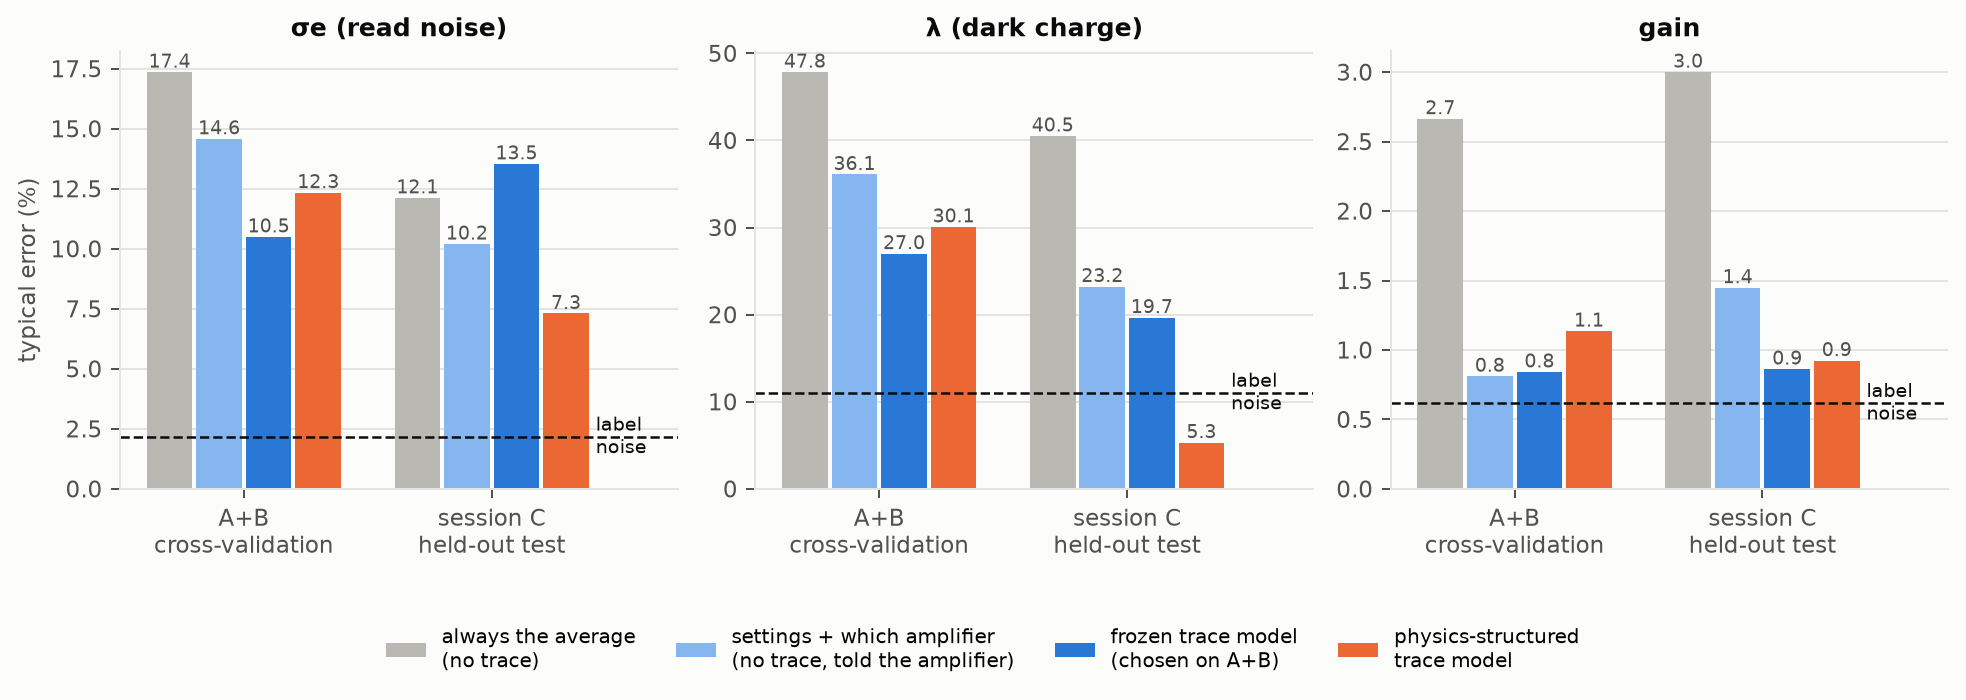
\includegraphics[width=\textwidth]{figures/fig1_traces_help.png}
\caption{Typical error (RMS of $\log$(predicted/true)) of the two baselines and two trace models, on the A+B
cross-validation and on the held-out session C. Frozen choice (made on A+B before C was looked at): $\sigma_e$
gp\_dim [P+A1], $\lambda$ pretrained [all], gain gp\_dim [P]. Physics-structured: physics\_white [P+A] for
$\sigma_e$, physics [all] for $\lambda$, physics [P] for the gain, the sets the A+B cross-validation chose (one model:
the $\lambda$ and gain parts of physics and physics\_white are the same). Light blue: the better of the GP and the
boosted trees on the settings and the amplifier's one-hot code (definitions in Appendix~\ref{app:models}). Dashed: the label noise (repeat scatter of the
labels over the four nominal packets).}
\label{fig:help}
\end{figure}

\section{The data}

\begin{itemize}
\item 43 planned packets in one night (sessions A: timing, B: one voltage at a time, C: joint changes), each with 5
  reference and 10 new trace sets ($2\times5$ pixels, 500 skips, 4 channels) and one $16\times1000\times500$ image.
\item \textbf{Settings:} every packet's reference traces were at nominal (the board-reset fix worked) and every
  requested change arrived in the traces and the image (VSUB reads back the potentiometer step, $\sim$0.2\,V high).
\item \textbf{Traces:} 2370 of 2580 board-101 traces usable ($\sim$8\,\% damaged). L1\_37, L1\_40 and L1\_41
  (session C) lost \emph{all} 40 traces at their own settings; such rows are now excluded automatically
  (\texttt{trace\_ok}, a rule on the traces only). Session C is reported both without them (main numbers) and with them.
\item \textbf{Labels} (run\_WADERs; \texttt{--all-ext} so ch3 is fitted too): 127 of 128 A+B labels usable. Repeat
  scatter at nominal (4 packets): $\sigma_e$ 2.2\,\%, gain 0.6\,\%, $\lambda$ 11\,\% (it drifted down over the night,
  Fig.~\ref{fig:night}).
\item \textbf{Drift correction (found and fixed):} the along-row drift correction, calibrated on the October images,
  inflated session-A $\sigma_e$ labels up to $\times3$ (L1\_06 ch0 0.145\,$\to$\,0.348\,e$^-$) and raised $\lambda$ by
  7--10\,\% on every channel; the raw images fit well ($\chi^2$/ndf 0.8--1.3), and the replicate pair L1\_06/L1\_23
  agrees on them (0.145/0.144). It is off for these data.
\end{itemize}

\section{Method}

\begin{itemize}
\item No model is told which amplifier it sees (label-free), except the references marked as such.
\item \textbf{Baselines:} the training average; a GP on the settings; and new, \emph{settings + amplifier identity}
  (GP or boosted trees on the settings and a one-hot of the amplifier, no trace). A trace model that does not beat the
  last one has learned nothing from the traces beyond which amplifier they come from.
\item \textbf{Validation:} cross-validation on A+B grouped by setting (packets at identical settings share a fold),
  packet bootstrap for intervals and paired comparisons; feature tiers frozen (label-free) before training; the model
  choice frozen in git (commit 25384b9) before session C was scored once.
\item \textbf{New:} \texttt{physics\_white}, the physics-structured model with the trace's white noise per skip as its
  noise term instead of the Allan-curve floor, which jumped between packets at the same setting ($\times1.45$ vs
  $\times1.17$).
\end{itemize}

\section{Results}

\begin{figure}[h]
\centering
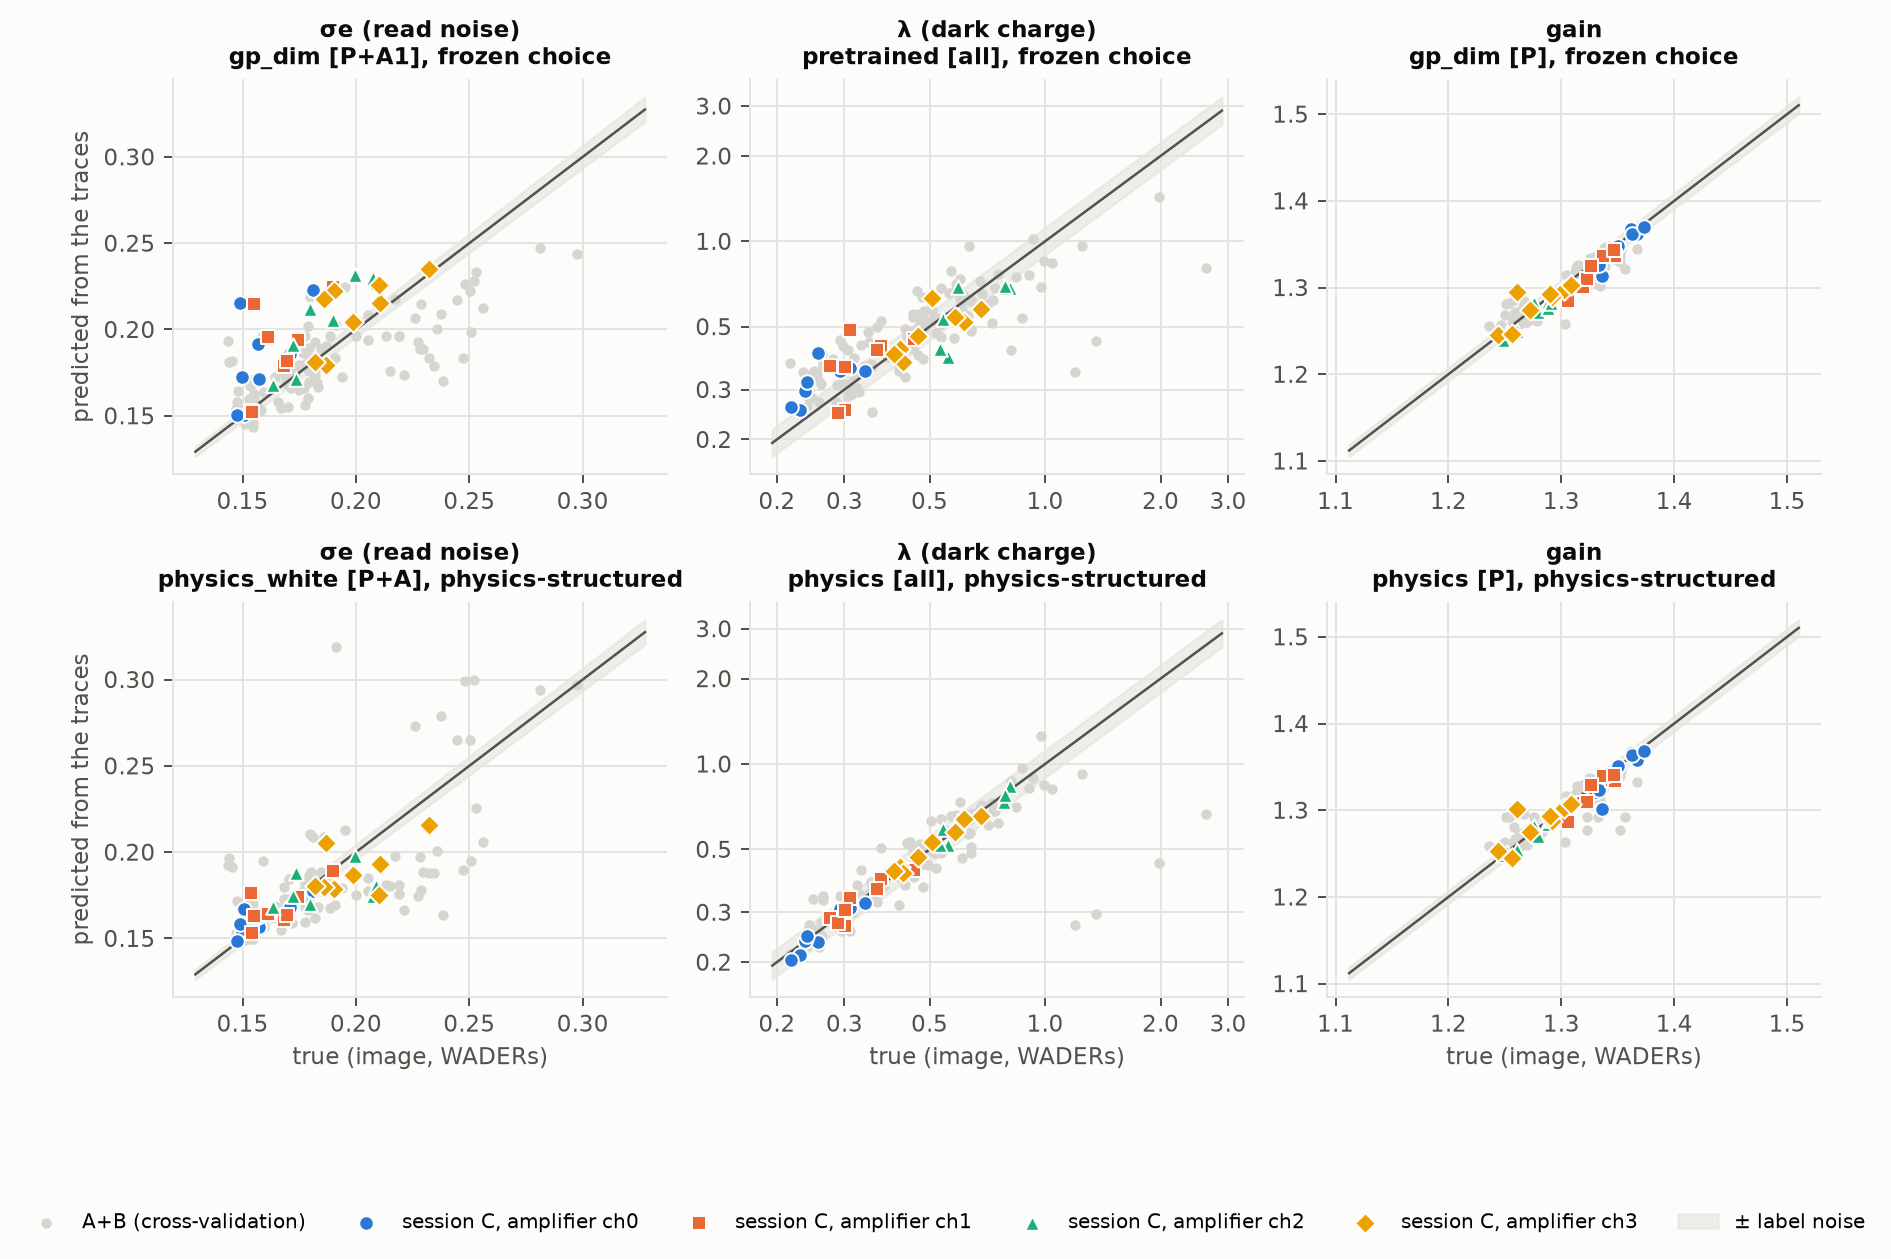
\includegraphics[width=\textwidth]{figures/fig2_session_c.png}
\caption{Session C, predicted vs true. Top: the frozen choice; bottom: the physics-structured models. Grey: the A+B
rows (cross-validation); coloured: the held-out session C, one marker per amplifier. Band: $\pm$ the label noise.}
\label{fig:c}
\end{figure}

\paragraph{Session C, paired against settings + amplifier (trees), packet bootstrap (8 packets).}
Each model at the feature set chosen on A+B (all models: Table~\ref{tab:all}).
$\lambda$: physics [all] 5.3 vs 23.2\,\%, $-17.9$ [$-25.8$, $-10.1$]; cnn [all] $-10.3$ [$-18.9$, $-1.6$]; frozen
pretrained $-3.6$ [$-14.4$, $+7.4$]. Gain: physics [P] 0.9 vs 1.4\,\%, $-0.5$ [$-1.3$, $+0.3$]; ridge [P+A1] $-0.7$
[$-1.1$, $-0.1$]; deep\_kernel [P+A1] $-0.7$ [$-1.3$, $-0.1$]; trees [P+A+B] $-0.4$ [$-0.6$, $-0.1$]; frozen gp\_dim
$-0.6$ [$-1.2$, $+0.1$]. $\sigma_e$: physics\_white [P+A] 7.3 vs 10.2\,\%, $-2.9$ [$-9.3$, $+3.1$]; frozen gp\_dim
$+3.3$ [$-2.9$, $+10.4$]. With the three packets without usable traces included,
physics\_white's $\sigma_e$ error is 27.5\,\% (51\,\% on those three packets alone): a model cannot predict from traces
that do not exist.

\paragraph{On A+B (cross-validation),} against settings + amplifier: $\lambda$ improves by 7--15 points for every
trace model (significant), $\sigma_e$ by 2--5 points (significant for gp\_dim only), the gain not at all (0.8 vs
0.8\,\%): on A+B the traces act for the gain as an amplifier fingerprint.

\begin{table}[h]
\centering\small
\caption{Session C error (\%) of every model at every trace-feature set (trained once on A+B; 8 packets, 32 rows).
Bold: each model's best set (chosen after the fact, so optimistic).}
\label{tab:c}
\begin{tabular}{lrrrrrr}
\toprule
model & none & P (8) & +A1 (44) & +A2 (81) & +B (96) & all (141) \\
\midrule
\multicolumn{7}{l}{\textbf{$\sigma_e$} \quad baselines: average 12.1, settings 11.5, settings + amplifier 10.2} \\ \midrule
physics\_white & 7.0 & \textbf{5.4} & 5.6 & 7.3 & 7.4 & 7.0 \\
physics & 25.7 & 28.2 & \textbf{24.5} & 29.7 & 29.1 & 29.0 \\
physics\_joint & 25.7 & 28.2 & \textbf{24.5} & 29.7 & 29.1 & 29.0 \\
sets & 11.0 & 10.7 & \textbf{10.3} & 11.1 & 11.5 & 12.5 \\
trees & 13.9 & \textbf{8.7} & 14.3 & 15.3 & 15.3 & 15.1 \\
gp & 11.5 & 11.2 & 12.0 & \textbf{10.5} & 12.1 & 12.1 \\
gp\_dim & 14.6 & 14.3 & \textbf{13.5} & 17.6 & 18.6 & 22.2 \\
nn & 11.3 & 10.0 & \textbf{5.9} & 10.9 & 11.6 & 11.5 \\
cnn & 10.8 & 11.2 & 12.7 & \textbf{8.4} & 10.0 & 8.6 \\
pretrained & 16.1 & 22.2 & 20.3 & 14.0 & 12.2 & \textbf{11.1} \\
deep\_kernel & 13.8 & \textbf{12.4} & 14.8 & 14.1 & 14.9 & 15.5 \\
ridge & 12.0 & \textbf{7.4} & 13.3 & 22.3 & 20.1 & 25.8 \\
\midrule
\multicolumn{7}{l}{\textbf{$\lambda$} \quad baselines: average 40.5, settings 40.2, settings + amplifier 23.2} \\ \midrule
physics\_white & 38.7 & 6.3 & 5.7 & \textbf{5.3} & 6.7 & 5.3 \\
physics & 38.7 & 6.3 & 5.7 & \textbf{5.3} & 6.7 & 5.3 \\
physics\_joint & 38.8 & 21.9 & \textbf{14.7} & 29.1 & 29.8 & 28.9 \\
sets & 38.7 & 6.3 & 5.7 & \textbf{5.3} & 6.7 & 5.3 \\
trees & 41.2 & 24.6 & 28.5 & 27.5 & 25.2 & \textbf{20.9} \\
gp & 40.2 & \textbf{33.6} & 34.9 & 34.7 & 40.5 & 40.5 \\
gp\_dim & 39.7 & 19.0 & \textbf{14.4} & 52.4 & 59.3 & 63.1 \\
nn & 38.9 & 22.7 & 13.6 & \textbf{12.5} & 14.6 & 13.5 \\
cnn & 20.2 & 18.9 & 15.5 & 13.9 & 14.5 & \textbf{12.9} \\
pretrained & 32.8 & 32.7 & 30.6 & 27.6 & 22.2 & \textbf{19.7} \\
deep\_kernel & 40.7 & 53.7 & \textbf{10.0} & 13.3 & 12.2 & 15.7 \\
ridge & 38.8 & 24.3 & \textbf{19.1} & 83.0 & 76.1 & 48.9 \\
\midrule
\multicolumn{7}{l}{\textbf{gain} \quad baselines: average 3.0, settings 3.0, settings + amplifier 1.4} \\ \midrule
physics\_white & 3.0 & 0.9 & \textbf{0.6} & 1.7 & 1.7 & 1.8 \\
physics & 3.0 & 0.9 & \textbf{0.6} & 1.7 & 1.7 & 1.8 \\
physics\_joint & 3.0 & 0.9 & \textbf{0.6} & 1.7 & 1.7 & 1.8 \\
sets & 3.0 & 0.9 & \textbf{0.6} & 1.7 & 1.7 & 1.8 \\
trees & 2.9 & 1.1 & \textbf{1.1} & 1.1 & 1.1 & 1.1 \\
gp & 3.0 & 2.5 & \textbf{2.4} & 2.4 & 3.0 & 3.0 \\
gp\_dim & 2.8 & \textbf{0.9} & 0.9 & 1.8 & 2.1 & 2.1 \\
nn & 2.8 & 1.0 & 0.8 & \textbf{0.7} & 0.9 & 1.0 \\
cnn & 1.1 & 1.1 & 1.0 & 1.0 & 1.2 & \textbf{1.0} \\
pretrained & 2.7 & 1.9 & 1.8 & \textbf{1.3} & 1.5 & 1.6 \\
deep\_kernel & 2.5 & 0.8 & \textbf{0.7} & 0.8 & 0.9 & 0.9 \\
ridge & 2.9 & 1.3 & \textbf{0.8} & 2.5 & 1.6 & 1.0 \\
\bottomrule
\end{tabular}

\end{table}

\begin{figure}[h]
\centering
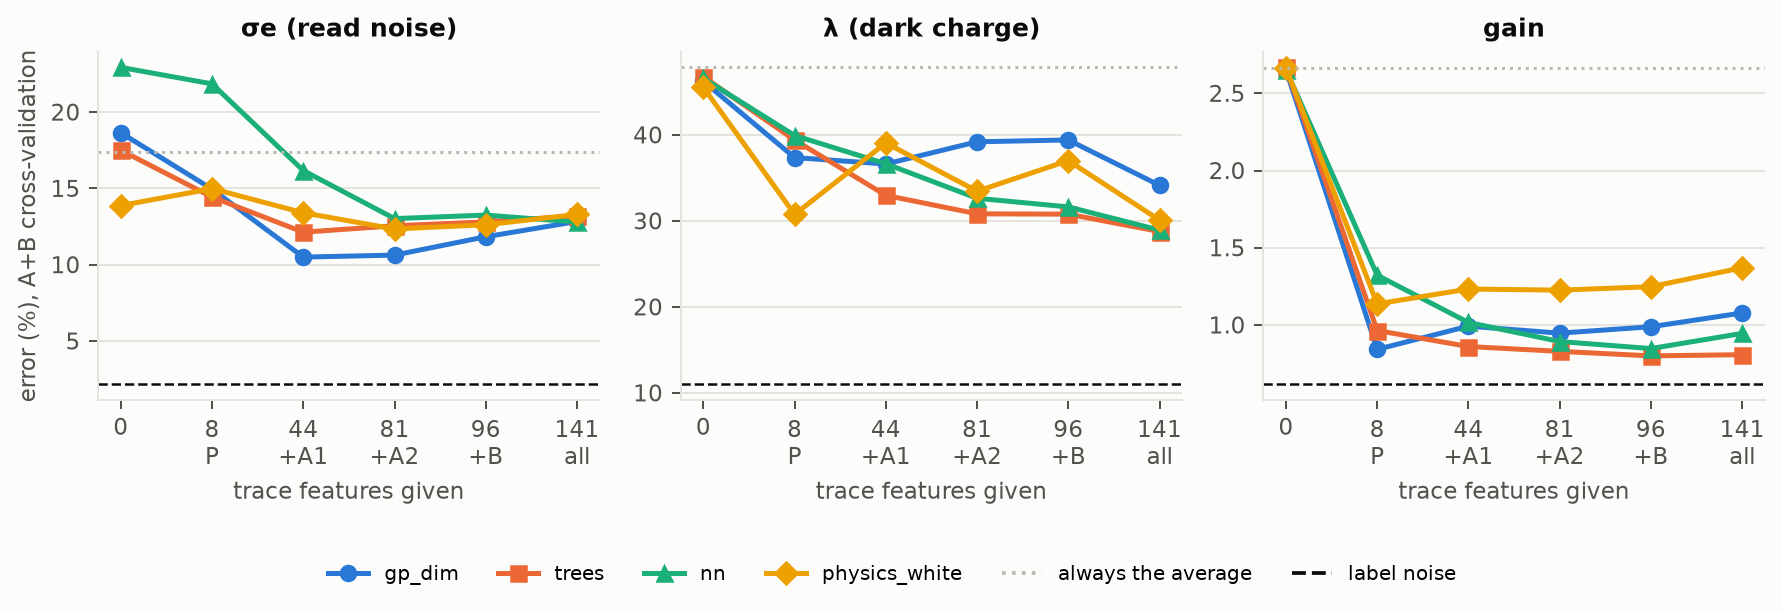
\includegraphics[width=\textwidth]{figures/fig6_ladder.png}
\caption{Error against the number of trace features given (A+B cross-validation, the evidence-tier order). The plain
models gain little beyond the 8 protected estimators (P) for the gain; $\sigma_e$ and $\lambda$ improve up to
$\sim$50--140 features for trees and the networks; with 32 packets the differences between sets are within the noise.}
\label{fig:ladder}
\end{figure}

\section{Every model at a glance}
\label{sec:glance}

Each model's exact definition, its fitted parameters and what it relies on are in Appendix~\ref{app:models}; this
section summarizes them. Every model is shown at the trace-feature set its A+B cross-validation chose, per target.

\begin{figure}[h]
\centering
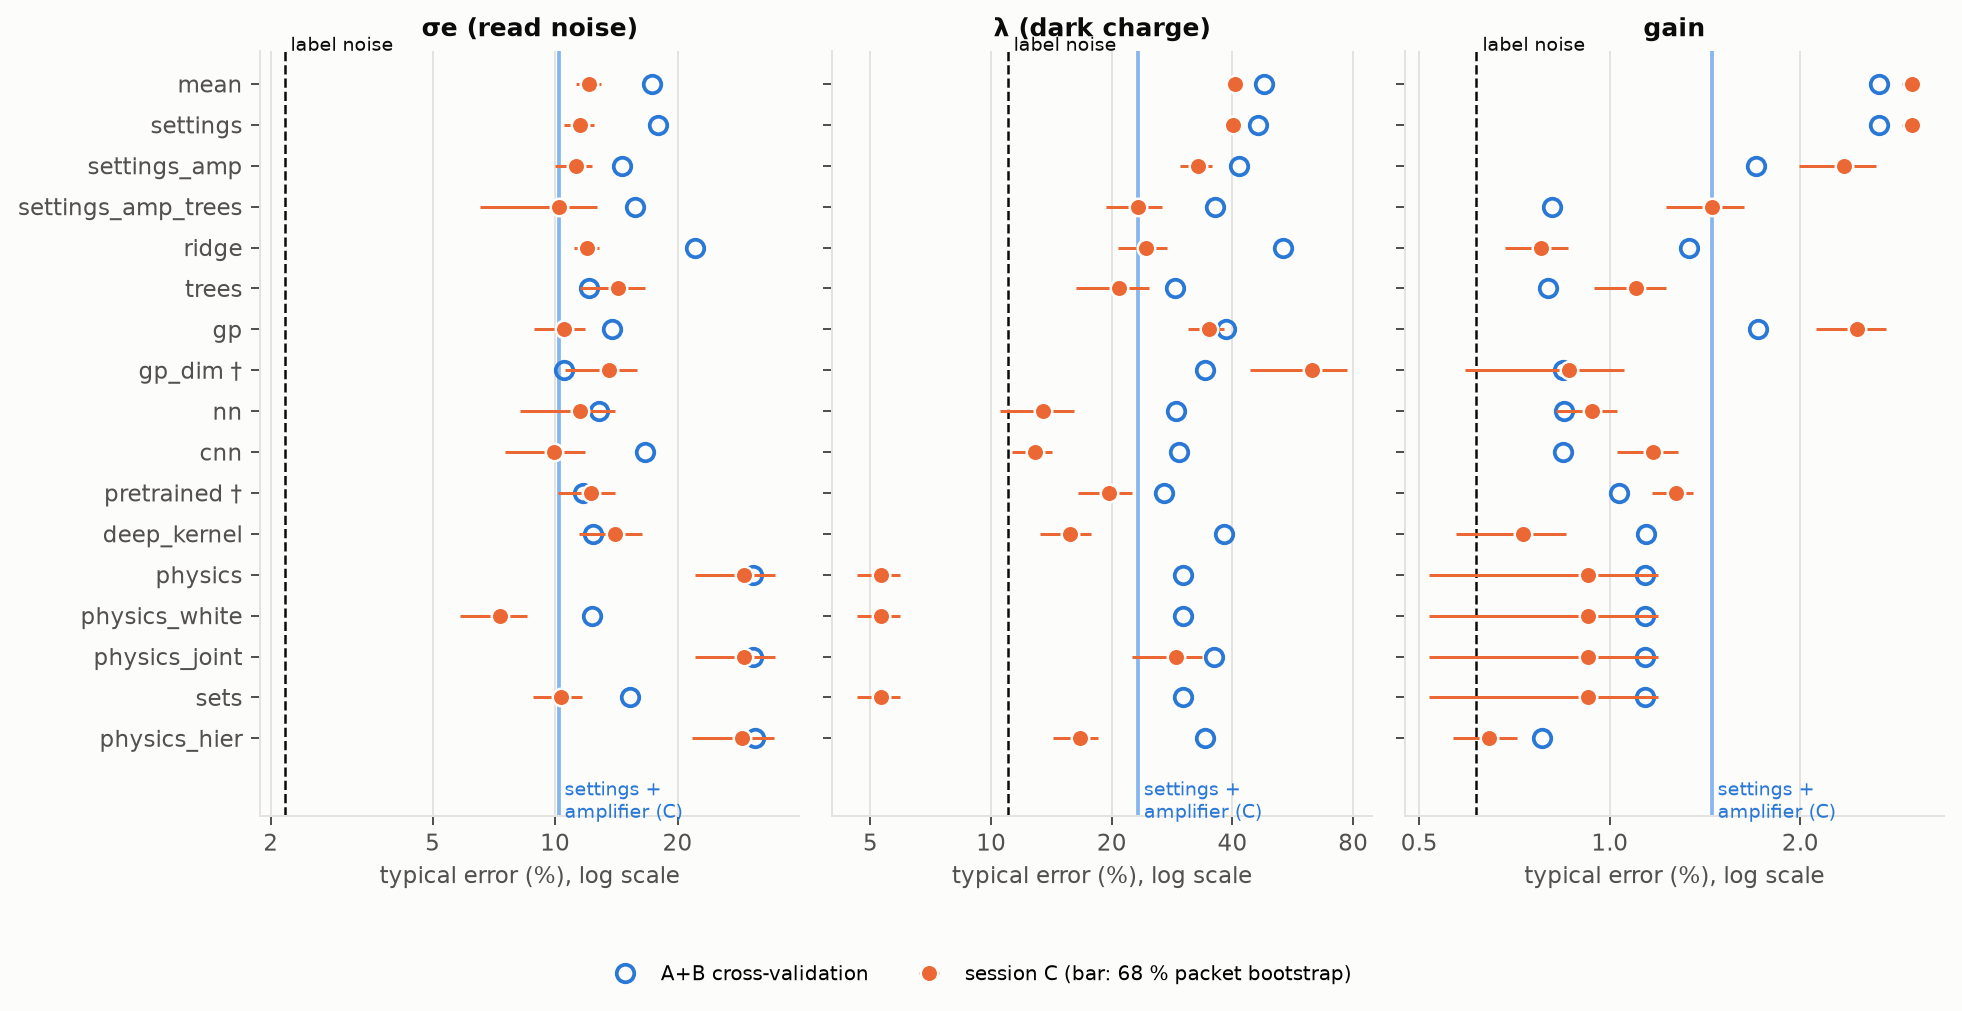
\includegraphics[width=\textwidth]{figures/fig7_all_models.png}
\caption{Every model's error: A+B cross-validation (open) and session C (filled, with the 68\,\% packet-bootstrap
interval), log scale. Vertical lines: settings + amplifier (trees) on session C, and the label noise. $\dagger$: the
frozen choice. The physics models share their $\lambda$ and gain parts.}
\label{fig:all}
\end{figure}

\begin{table}[h]
\centering\scriptsize\renewcommand{\arraystretch}{0.92}
\caption{Every model at the feature set chosen on A+B: errors (\%) and the paired session C difference from settings
+ amplifier (trees), in percentage points with its 95\,\% packet-bootstrap interval (bold: excludes zero), and the
fraction of resamples in which the model is better. $\dagger$: frozen choice.}
\label{tab:all}
\begin{tabular}{llrrrl}
\toprule
model & set (chosen on A+B) & A+B CV & session C & C $-$ settings + amp. [95\,\%] & P(better) \\
\midrule
\multicolumn{6}{l}{\textbf{$\sigma_e$} \quad error in \%; reference: settings + amplifier (trees)} \\
\midrule
\texttt{mean} & none & 17.4 & 12.1 & +1.9 [-2.9, +6.8] & 0.20 \\
\texttt{settings} & none & 17.9 & 11.5 & +1.3 [-3.2, +6.1] & 0.26 \\
\texttt{settings\_amp} & none & 14.6 & 11.2 & +1.0 [-3.6, +6.0] & 0.30 \\
\texttt{settings\_amp\_trees} & none & 15.7 & 10.2 & reference &  \\
\texttt{ridge} & none & 22.0 & 12.0 & +1.8 [-3.4, +6.7] & 0.23 \\
\texttt{trees} & P+A1 & 12.1 & 14.3 & \textbf{+4.1 [+0.6, +9.3]} & 0.01 \\
\texttt{gp} & P+A & 13.8 & 10.5 & +0.3 [-4.1, +5.3] & 0.41 \\
\texttt{gp\_dim}$^{\dagger}$ & P+A1 & 10.5 & 13.5 & +3.3 [-2.9, +10.4] & 0.16 \\
\texttt{nn} & all & 12.8 & 11.5 & +1.3 [-4.7, +8.3] & 0.34 \\
\texttt{cnn} & P+A+B & 16.6 & 10.0 & -0.2 [-3.5, +4.4] & 0.55 \\
\texttt{pretrained} & P+A+B & 11.7 & 12.2 & +2.0 [-2.0, +7.3] & 0.17 \\
\texttt{deep\_kernel} & P+A & 12.4 & 14.1 & +3.9 [-4.3, +11.2] & 0.14 \\
\texttt{physics} & P+A+B & 30.6 & 29.1 & \textbf{+18.9 [+9.2, +30.2]} & 0.00 \\
\texttt{physics\_white} & P+A & 12.3 & 7.3 & -2.9 [-9.3, +3.1] & 0.74 \\
\texttt{physics\_joint} & P+A+B & 30.6 & 29.1 & \textbf{+18.9 [+9.2, +30.2]} & 0.00 \\
\texttt{sets} & P+A1 & 15.3 & 10.3 & +0.1 [-6.9, +6.2] & 0.43 \\
\texttt{physics\_hier} & P+A & 31.0 & 28.8 & \textbf{+18.6 [+7.7, +29.6]} & 0.00 \\
\midrule
\multicolumn{6}{l}{\textbf{$\lambda$} \quad error in \%; reference: settings + amplifier (trees)} \\
\midrule
\texttt{mean} & none & 47.8 & 40.5 & \textbf{+17.3 [+9.4, +25.7]} & 0.00 \\
\texttt{settings} & none & 46.4 & 40.2 & \textbf{+17.0 [+9.0, +25.5]} & 0.00 \\
\texttt{settings\_amp} & none & 41.6 & 32.8 & +9.5 [-0.4, +19.5] & 0.03 \\
\texttt{settings\_amp\_trees} & none & 36.1 & 23.2 & reference &  \\
\texttt{ridge} & P & 53.5 & 24.3 & +1.1 [-10.9, +12.9] & 0.42 \\
\texttt{trees} & all & 28.8 & 20.9 & -2.3 [-16.7, +10.8] & 0.63 \\
\texttt{gp} & P+A1 & 38.6 & 34.9 & \textbf{+11.7 [+1.0, +22.6]} & 0.01 \\
\texttt{gp\_dim} & all & 34.1 & 63.1 & +39.9 [-2.5, +70.7] & 0.04 \\
\texttt{nn} & all & 28.9 & 13.5 & -9.7 [-19.8, +0.1] & 0.97 \\
\texttt{cnn} & all & 29.4 & 12.9 & \textbf{-10.3 [-18.9, -1.6]} & 0.99 \\
\texttt{pretrained}$^{\dagger}$ & all & 27.0 & 19.7 & -3.6 [-14.4, +7.4] & 0.74 \\
\texttt{deep\_kernel} & all & 38.1 & 15.7 & -7.5 [-17.1, +2.3] & 0.93 \\
\texttt{physics} & all & 30.1 & 5.3 & \textbf{-17.9 [-25.8, -10.1]} & 1.00 \\
\texttt{physics\_white} & all & 30.1 & 5.3 & \textbf{-17.9 [-25.8, -10.1]} & 1.00 \\
\texttt{physics\_joint} & all & 35.9 & 28.9 & +5.7 [-8.6, +19.4] & 0.25 \\
\texttt{sets} & all & 30.1 & 5.3 & \textbf{-17.9 [-25.8, -10.1]} & 1.00 \\
\texttt{physics\_hier} & P & 34.1 & 16.6 & -6.6 [-14.8, +1.1] & 0.96 \\
\midrule
\multicolumn{6}{l}{\textbf{gain} \quad error in \%; reference: settings + amplifier (trees)} \\
\midrule
\texttt{mean} & none & 2.7 & 3.0 & \textbf{+1.6 [+1.3, +1.9]} & 0.00 \\
\texttt{settings} & none & 2.7 & 3.0 & \textbf{+1.6 [+1.3, +1.9]} & 0.00 \\
\texttt{settings\_amp} & none & 1.7 & 2.3 & \textbf{+0.9 [+0.5, +1.3]} & 0.00 \\
\texttt{settings\_amp\_trees} & none & 0.8 & 1.4 & reference &  \\
\texttt{ridge} & P+A1 & 1.3 & 0.8 & \textbf{-0.7 [-1.1, -0.1]} & 0.99 \\
\texttt{trees} & P+A+B & 0.8 & 1.1 & \textbf{-0.4 [-0.6, -0.1]} & 0.99 \\
\texttt{gp} & P & 1.7 & 2.5 & \textbf{+1.0 [+0.5, +1.4]} & 0.00 \\
\texttt{gp\_dim}$^{\dagger}$ & P & 0.8 & 0.9 & -0.6 [-1.2, +0.1] & 0.95 \\
\texttt{nn} & P+A+B & 0.8 & 0.9 & -0.5 [-1.0, +0.0] & 0.97 \\
\texttt{cnn} & P+A+B & 0.8 & 1.2 & -0.3 [-0.7, +0.3] & 0.84 \\
\texttt{pretrained} & P+A & 1.0 & 1.3 & -0.2 [-0.5, +0.3] & 0.78 \\
\texttt{deep\_kernel} & P+A1 & 1.1 & 0.7 & \textbf{-0.7 [-1.3, -0.1]} & 0.99 \\
\texttt{physics} & P & 1.1 & 0.9 & -0.5 [-1.3, +0.3] & 0.88 \\
\texttt{physics\_white} & P & 1.1 & 0.9 & -0.5 [-1.3, +0.3] & 0.88 \\
\texttt{physics\_joint} & P & 1.1 & 0.9 & -0.5 [-1.3, +0.3] & 0.88 \\
\texttt{sets} & P & 1.1 & 0.9 & -0.5 [-1.3, +0.3] & 0.88 \\
\texttt{physics\_hier} & P+A1 & 0.8 & 0.6 & \textbf{-0.8 [-1.1, -0.5]} & 1.00 \\
\bottomrule
\end{tabular}

\end{table}

\begin{figure}[h]
\centering
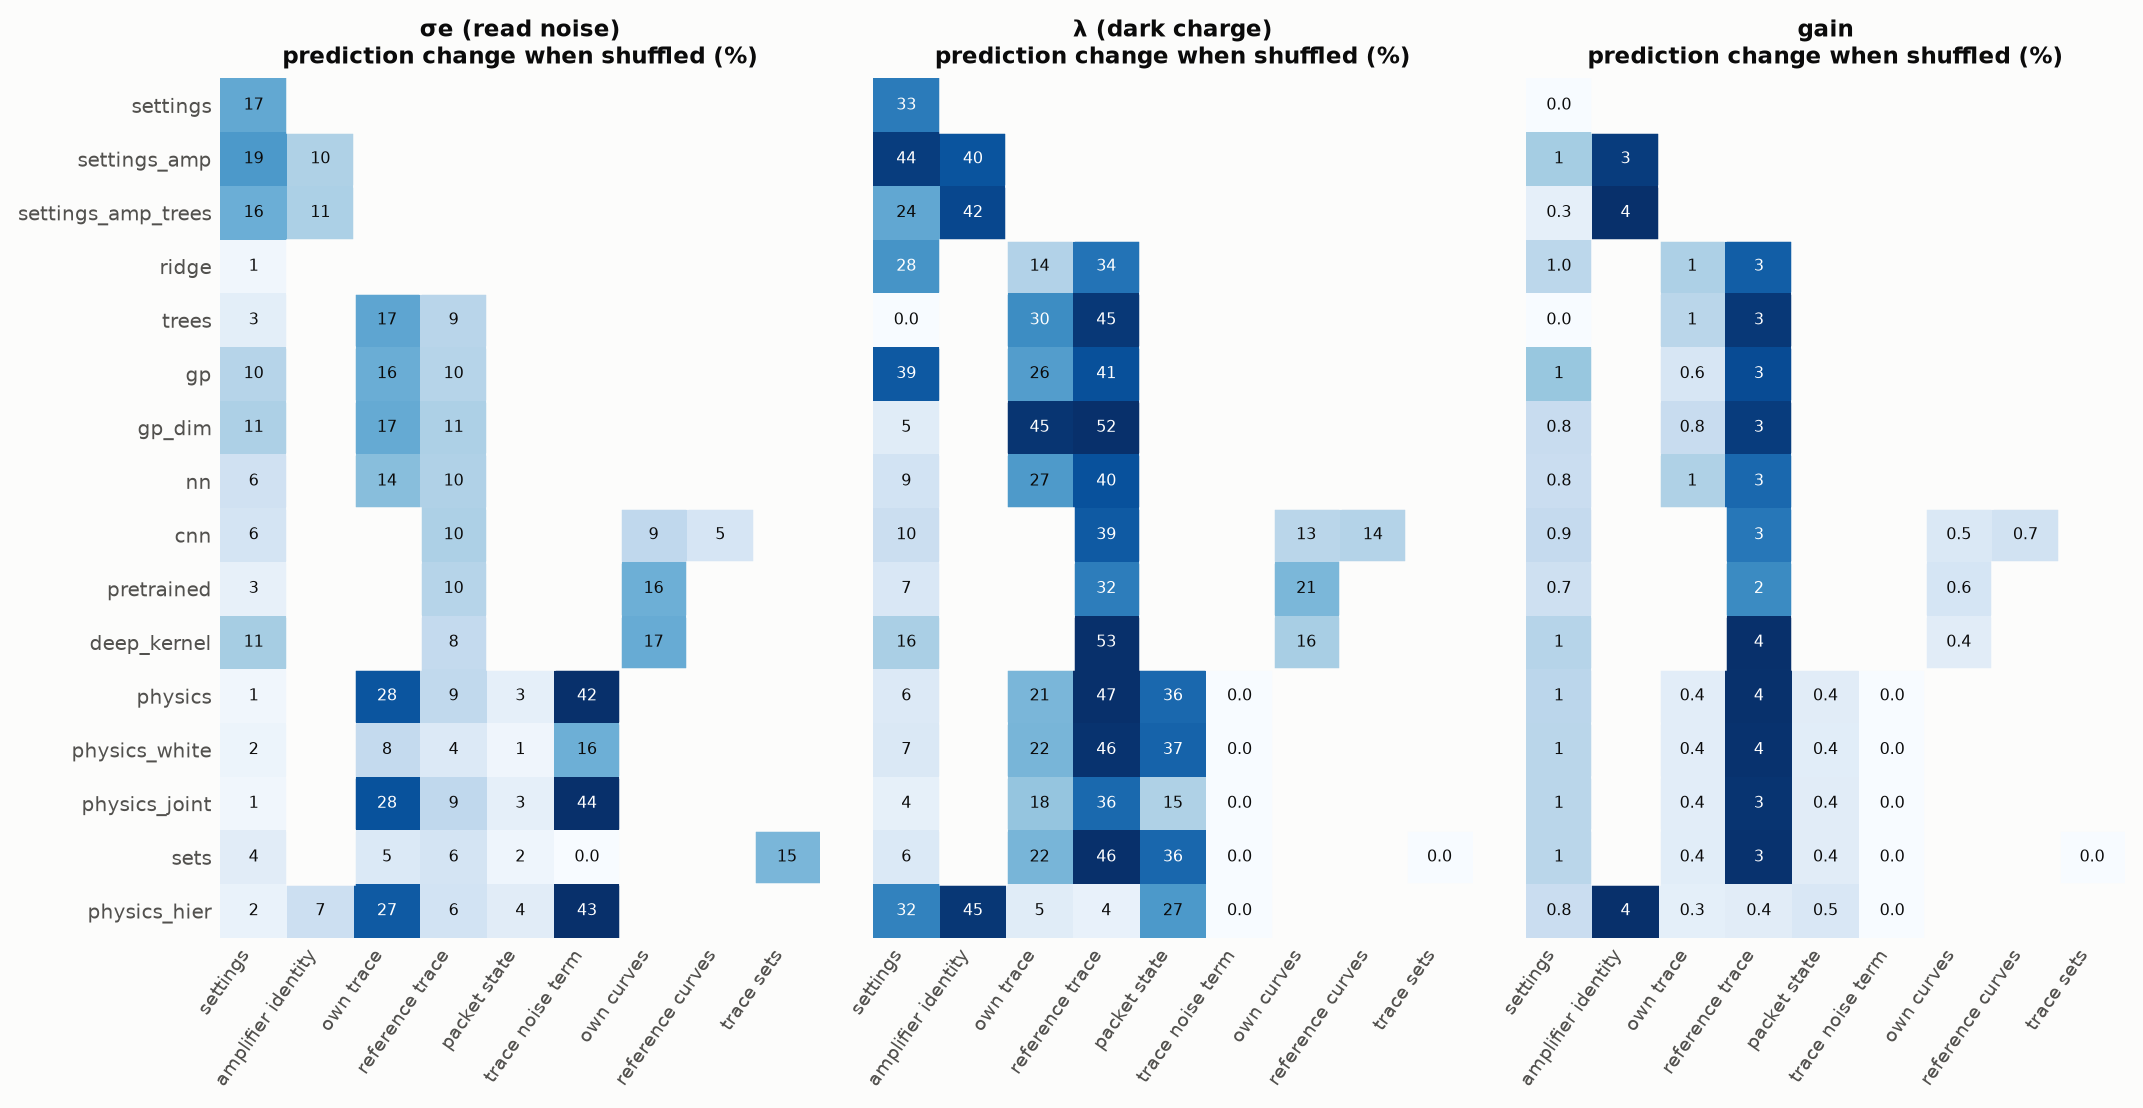
\includegraphics[width=\textwidth]{figures/fig8_reliance.png}
\caption{What every model's predictions move with: the RMS change of the prediction (\% of the target) when one group
of inputs is shuffled across all rows (A+B and C), the model fitted once on A+B. Blank: the model does not see that
group. The trace noise term is used only for $\sigma_e$ by construction.}
\label{fig:reliance}
\end{figure}

\paragraph{What the models rely on} (Fig.~\ref{fig:reliance}; per model, Appendix~\ref{app:models}).
\begin{itemize}
\item \textbf{The gain comes from recognising the amplifier.} Every trace model's gain rests on the reference trace's
  noise features (jump-robust CDS $\sigma$, white noise per skip, null-CDS noise). Shuffled across all rows they move
  the gain by about 3.5\,\%; shuffled only among rows of the same amplifier, by about 0.5\,\%. So the traces tell the
  models \emph{which amplifier} this is, and the gain follows. The settings move it by about 1\,\% (VDD, VR, VDRAIN). The
  gain varies little within an amplifier (repeat scatter 0.6\,\%), so this is most of what there is to learn.
\item \textbf{$\lambda$: the amplifier, the own trace, and the CCD's state.} In the physics family's $\lambda$ GP (the
  best $\lambda$ model, 5.3\,\%) the reference trace moves $\lambda$ by 46\,\% but by only 6\,\% within an amplifier: it
  identifies the amplifier, and shuffling it costs 46 points on C. The own trace moves it by 22\,\% also within an
  amplifier and costs 18 points on C: it carries information about this packet beyond the amplifier. The packet state
  moves the predictions by 37\,\% but costs nothing on C: what it learned about the CCD's drift in A+B does not carry
  over to session C. The settings move $\lambda$ by 6\,\%. The SAAS prior keeps few inputs, and a single one (the
  reference trace's edge jitter) moves $\lambda$ by 58\,\%: a fragile point for a new night.
\item \textbf{$\sigma_e$: the measured noise versus proxies.} \texttt{physics\_white}'s $\sigma_e$ rests on the trace's
  white noise (moves 16\,\%, costs 5 points on C when shuffled); its correction uses own-trace features
  (permutation entropy, line frequency, row-start ratio, transient time constant). The flexible models (gp\_dim,
  trees, nn) rely instead on own-trace timing proxies (row-start recovery time, CDS ringing in skips 1--4) and the
  settings, and never on a noise measurement directly; they fit the A+B timing packets and fail on C. \texttt{physics}
  leans on the Allan floor (42\,\%), the unstable term that gives it 29\,\%.
\item \textbf{The references.} The settings-only GP moves $\lambda$ with delayInt and the RG low levels and does not
  move the gain at all. settings + amplifier (trees) uses only five inputs: delayInt and the four amplifier columns.
  With at least 10 rows per leaf, a knob changed in one or two A+B packets can never be split on. The labelled
  \texttt{physics\_hier} predicts $\lambda$ from the amplifier identity (45\,\%) and the settings (32\,\%) and is worse on C
  (16.6\,\%) than the label-free physics model, which identifies the amplifier from its traces and also reads its state.
\end{itemize}

\begin{figure}[h]
\centering
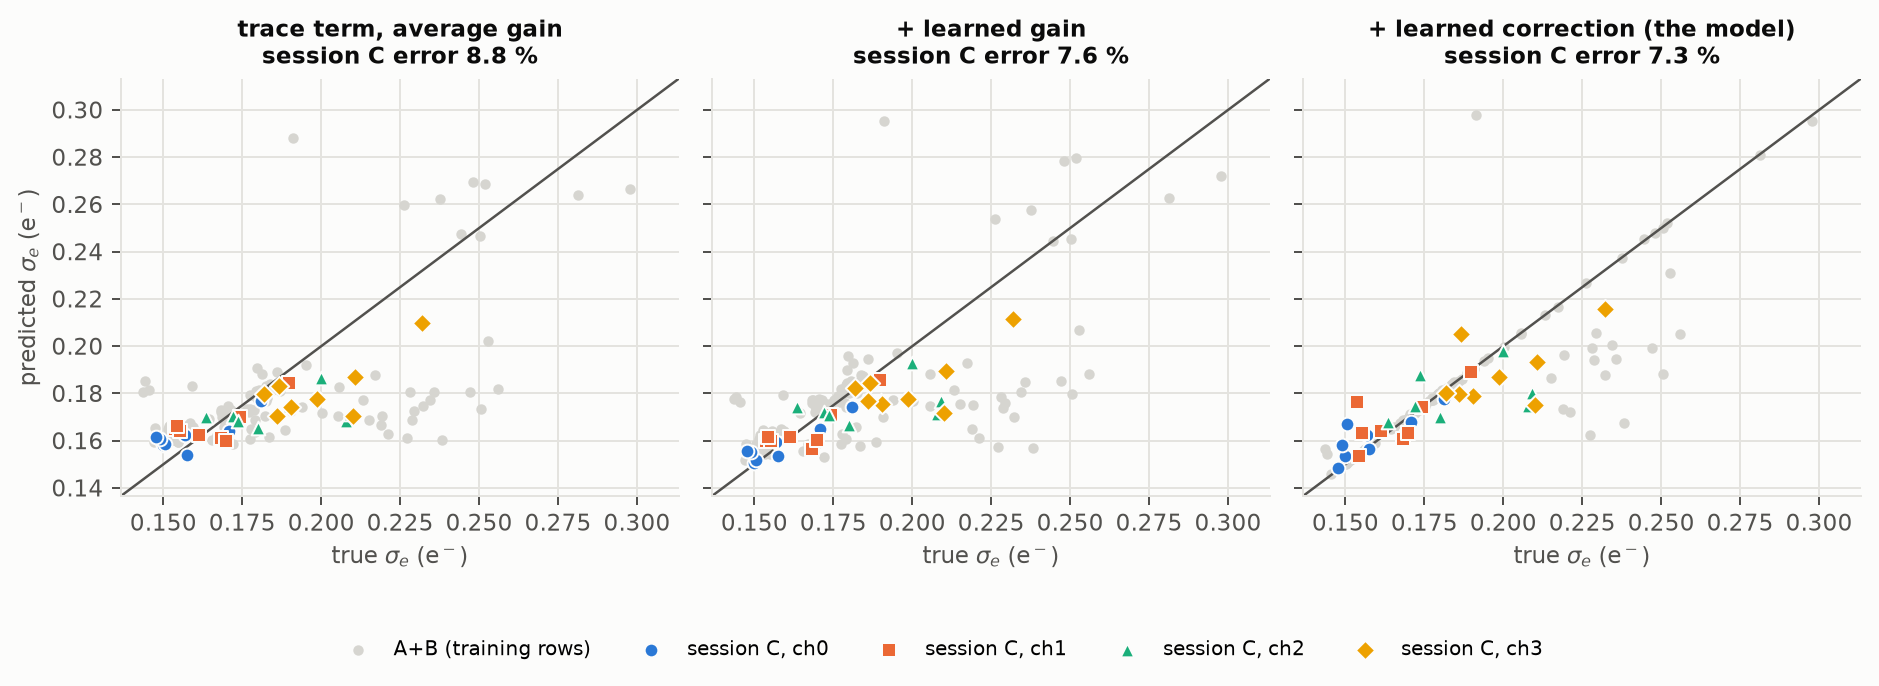
\includegraphics[width=\textwidth]{figures/fig9_physics_terms.png}
\caption{The physics-structured $\sigma_e$ (physics\_white [P+A]) built up term by term: the trace's white noise
$/\sqrt N$ divided by the average gain, then by the learned gain, then with the learned correction. Most of the
session C accuracy comes from the measured noise. In A+B (grey; training rows, so the right panel is in-sample) the
trace term alone misses the timing packets; the correction pulls them in.}
\label{fig:terms}
\end{figure}

\paragraph{Caveats.} Shuffling measures what a fitted model uses, not what is causally true; correlated inputs share
credit (hence the group shuffles). The network models were refitted for this analysis, and with their random starts
their session C errors differ from the scored run by up to 2 points (the tables report the scored run).


\section{Where the errors come from}

\begin{figure}[h]
\centering
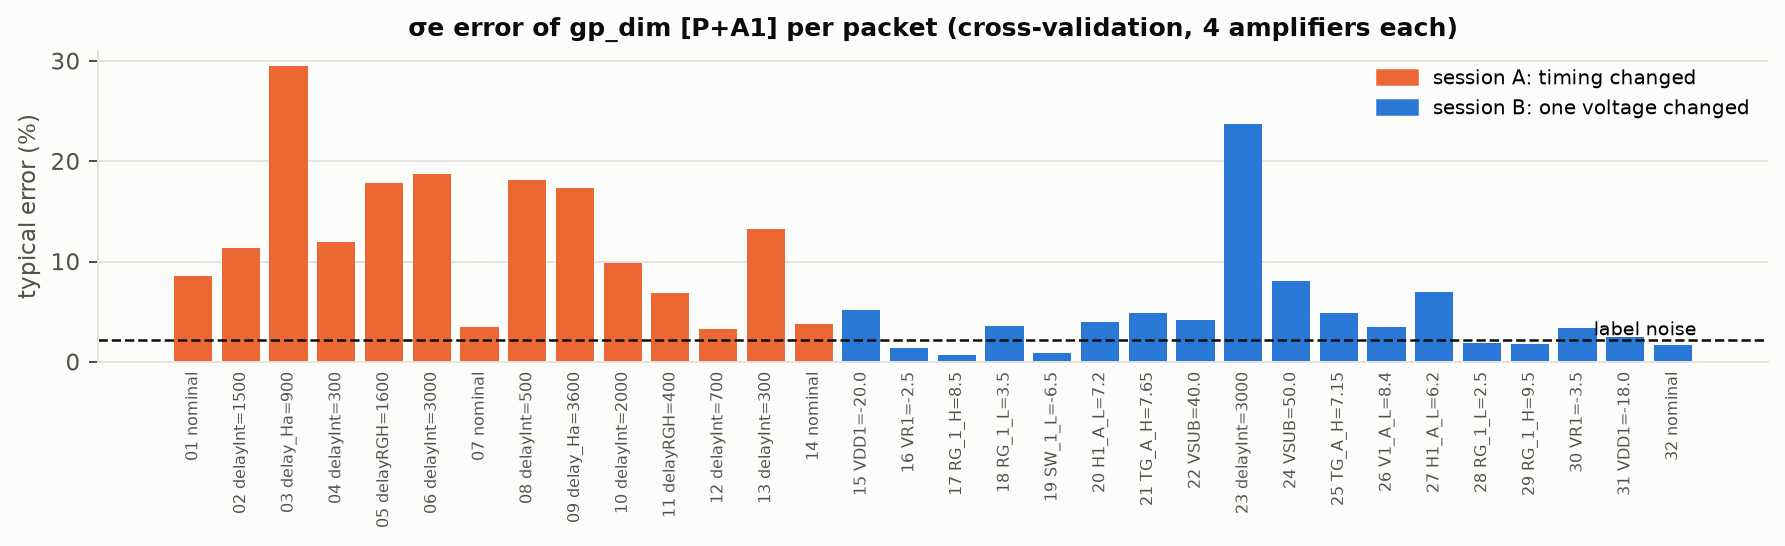
\includegraphics[width=\textwidth]{figures/fig3_sigma_error_by_packet.png}
\caption{$\sigma_e$ error of gp\_dim [P+A1] per A+B packet. Session A (timing) is 43\,\% of the rows but 76\,\% of
the squared error.}
\label{fig:pkt}
\end{figure}

\begin{figure}[h]
\centering
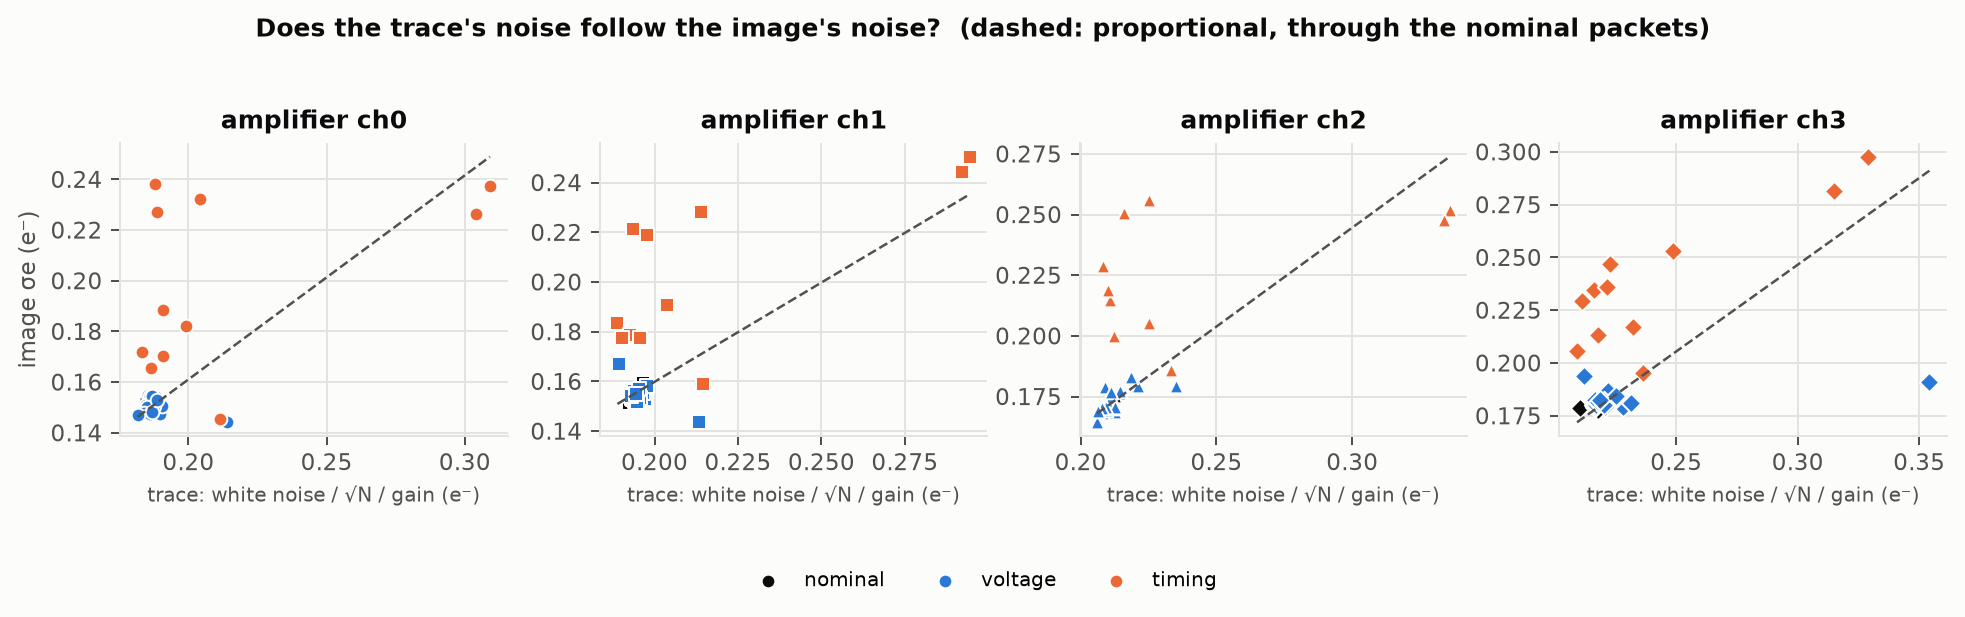
\includegraphics[width=\textwidth]{figures/fig4_trace_vs_image.png}
\caption{The trace's own noise estimate (white noise per skip $/\sqrt{N}/$gain) against the image's $\sigma_e$, per
amplifier. Voltage packets (blue) sit on the nominal proportionality; timing packets (orange) scatter off it: for them
the image's noise changes in ways the trace does not show.}
\label{fig:tvi}
\end{figure}

\begin{figure}[h]
\centering
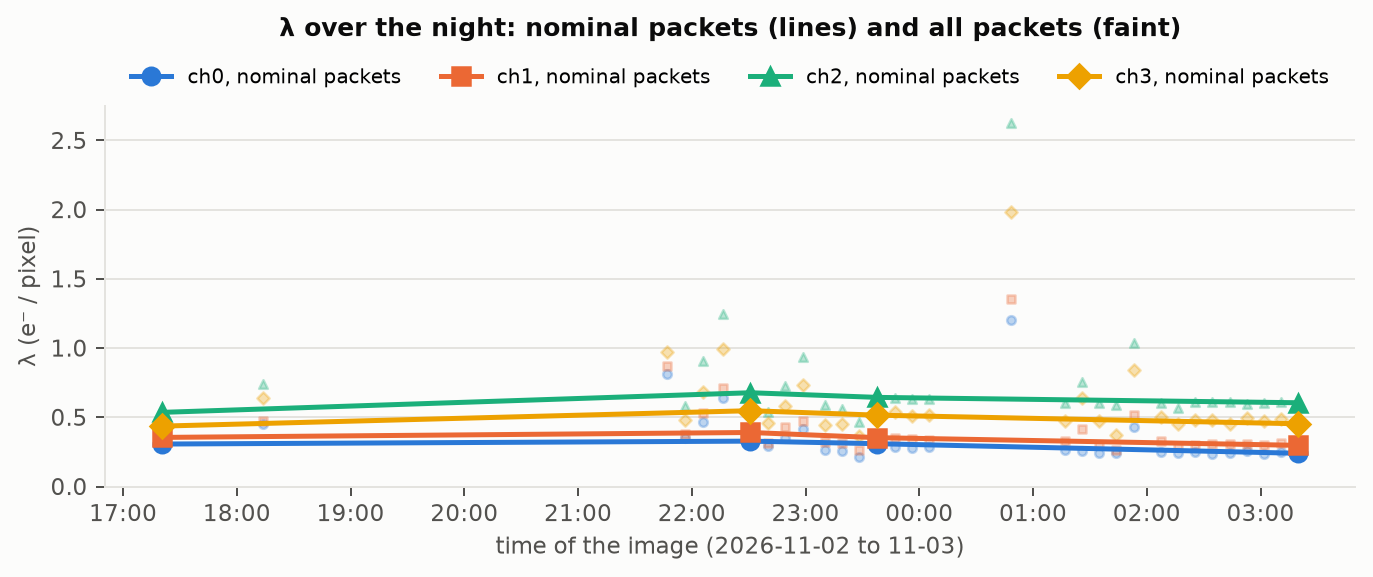
\includegraphics[width=0.85\textwidth]{figures/fig5_lambda_night.png}
\caption{$\lambda$ over the night. The nominal packets (lines) drift down by $\sim$20\,\%; the outliers near 00:50 are
L1\_18, whose queue stalled 38 minutes before its image with no flush in between.}
\label{fig:night}
\end{figure}

\begin{table}[h]
\centering\small
\caption{Assessment by cause.}
\label{tab:causes}
\begin{tabular}{p{2.3cm}p{6.6cm}p{6.3cm}}
\toprule
cause & what we found & status / remedy \\
\midrule
labels & drift correction corrupted session-A $\sigma_e$ and shifted $\lambda$ by 7--10\,\%; the ``CIC'' part of the
per-row split mixes serial-register charge (the overscan holds 70--85\,\% of the active $\lambda$) and charge collected
before the readout & correction off (fixed); the total $\lambda$ from WADERs stays the target; split into serial and
array parts tested and \emph{not} adopted (not better than direct) \\
data & 8\,\% of traces damaged; 3 C packets without any usable trace at their settings & excluded by rule; v2
safeguards retake damaged traces and restart a packet with more than 5 \\
procedure & $\lambda$ carries the CCD's history (night drift; time since the last flush, L1\_18); no flush between
traces and image & v2: flush right before the image, fixed timeline, nominal every 7 packets, 32-row image; log
temperature and time since clear \\
inputs (traces) & for timing changes the image's $\sigma_e$ moves in ways the $2\times5$-pixel trace does not follow;
10 pixels measure the pixel-to-pixel noise only to $\sim\pm24$\,\% & level-1 strips read like the image
(Section~\ref{sec:next}) \\
models & the Allan-floor noise term was unstable (fixed: physics\_white); CV on one-at-a-time packets chose flexible
models that did not generalise to joint changes & physics-structured model as default for $\lambda$ and gain;
choose models on joint-design data (v2) \\
\bottomrule
\end{tabular}
\end{table}

\section{How to proceed}
\label{sec:next}

\begin{enumerate}
\item \textbf{Take the v2 plan} (\texttt{lvl1/packet\_plan\_v2/}, \texttt{daq\_scripts/run\_plan.sh}): 76 packets in a
  joint Sobol design over 12 knob groups, so model choice and test both see joint changes; nominal every 7 packets;
  3 + 5 trace sets with automatic retakes and restarts; flush before and after the image; 32-row image.
\item \textbf{Three input sources on the same packets} (user, 2026-11-03): every packet also takes a level-1 strip
  (every skip of every pixel, all four channels, read exactly like the image: prescan 5300, register clear, 500
  skips) at the reference and at the new settings. The pipeline (reader \texttt{src/decode\_l1.py}, features
  \texttt{src/l1\_features.py}, and the input folders \texttt{model\_inputs}, \texttt{model\_inputs\_l1} and
  \texttt{model\_inputs\_both}) scores every model on (1) the traces, (2) the strip, (3) both, on the same rows and
  folds. Before the first v2
  night: a short DAQ test of the strip sizes ($1\times500$, $1\times1000$, $2\times1000$).
\item \textbf{Models:} the physics-structured model (white-noise term) as the default for $\lambda$ and gain; gp\_dim,
  trees and nn as challengers for $\sigma_e$; choose again on v2 with setting-grouped CV, freeze, and score session E
  once.
\item \textbf{After v2:} pool with these 40 packets (differences between nights as inputs), measure a learning curve
  (25--100\,\% of the packets) to see whether more packets still help.
\end{enumerate}

\appendix
% The models one by one: exact definitions (hand-written) and, per model, the generated tables
% (models/<model>.tex, lvl1/report_models.py, from lvl1/explain_models.py).

\section{The models in detail}
\label{app:models}

\subsection{Common notation}

\paragraph{Rows and targets.} One row $i$ is one amplifier $a(i)$ of board 101 in one packet $p(i)$. Each model predicts
three numbers per row, always in log space,
\[
y_i = \big(\log\sigma_{e,i},\ \log\lambda_i,\ \log g_i\big),
\]
with $\sigma_e$ in e$^-$, $\lambda$ in e$^-$/pixel and the gain $g$ in ADU/e$^-$, all from WADERs on the packet's image.
WADERs also gives each label's error $\delta_i$ (relative, so a variance $\delta_i^2$ in log units); only the
physics-structured models use it.

\paragraph{Inputs.} Four blocks exist; each model uses some of them:
\begin{itemize}
\item $\theta_i\in\mathbb R^{67}$: the packet's settings as the boards report them (sequencer delays, NPSD, NVWAIT,
  clock highs and lows, VSUB, VDD, VDRAIN, VR, offsets).
\item $u_i$: the \emph{own-trace} features: the trace features of amplifier $a(i)$ at the packet's settings, each the
  robust mean over the packet's new trace sets (values beyond $5\times1.4826$\,MAD of the median dropped).
\item $v_i$: the \emph{reference-trace} features: the same features of the same amplifier from the packet's reference
  trace sets, taken at nominal settings a few minutes earlier. They measure the amplifier and the CCD's state at that
  moment, not the setting.
\item $s_i$: the \emph{packet state} (physics models only): the reference features averaged over the amplifiers of the
  packet, each amplifier's own average removed first,
  \[ s_i=\frac{1}{|p(i)|}\sum_{j\in p(i)}\big(v_j-\bar v_{a(j)}\big),\qquad \bar v_a=\text{mean of }v\text{ over the rows of amplifier }a. \]
  It is the common, amplifier-free part of the reference traces: the CCD's drifting state.
\end{itemize}
A \emph{feature set} (P, P+A1, P+A, P+A+B, all; Section~\ref{sec:next} and the frozen tiers) chooses which trace
features enter $u_i$ and $v_i$; ``none'' leaves only $\theta_i$. Before any fit, on the training rows only: a column
with more than 20\,\% missing values or no variation is dropped (in A+B this drops every knob that changed only in the
test fold), and missing values are filled with the training median.

\paragraph{The amplifier.} No trace model is told which amplifier a row comes from: it sees that amplifier's own
traces. The exceptions are the references \texttt{settings\_amp}, \texttt{settings\_amp\_trees} and
\texttt{physics\_hier}.

\paragraph{Error.} With $\hat y_i$ the predicted log value of one target, the error is
$100\sqrt{\tfrac1n\sum_i(\hat y_i-y_i)^2}$\,\%, the typical relative error. \emph{A+B CV}: 5 folds of the 32 A+B
packets, packets at identical settings in the same fold, each fold predicted by a fit on the other four.
\emph{Session C}: one fit on all A+B rows, 32 C rows predicted. \emph{Paired difference}: the C error minus that of
settings + amplifier (trees), with a 95\,\% interval from 1000 bootstrap resamples of the 8 C packets (the same
resamples for both models); bold if it excludes zero.

\paragraph{Which feature set.} Each model is reported at the set with the lowest A+B CV error, separately per target
(chosen without looking at C). The frozen choice is marked $\dagger$.

\paragraph{What a model relies on} (lvl1/explain\_models.py). The model is fitted once on A+B and predicts every row.
Then one input, or one group $G$ of inputs, is shuffled: its values are moved between rows by a random permutation
$\pi$, the other inputs stay, and the model predicts again (no refit). Three numbers per group and target, each the
mean over 20 shuffles:
\[
S_G=100\sqrt{\tfrac1n\textstyle\sum_i\big(\hat y_i^{(\pi_G)}-\hat y_i\big)^2}\ \%,\qquad
L_G=\text{err}_C^{(\pi_G)}-\text{err}_C ,
\]
and $S_G^{\text{amp}}$, the same as $S_G$ with $\pi$ moving values only among rows of the same amplifier.
$S_G$ is how far the predictions move: what the model \emph{uses}, right or wrong. $S^{\text{amp}}_G$ keeps every
row's values within its own amplifier, so it removes what the inputs say about \emph{which} amplifier this is: if
$S^{\text{amp}}\ll S$, the model uses the group as an amplifier fingerprint. $L_G$ (shuffled among the C rows) is how
much the group \emph{helps} on new packets; it can be negative when a group misleads. Correlated inputs share credit:
shuffling one of two near-copies changes little, which is why groups are shuffled together.

\paragraph{Fitted parameters.} Where a model has interpretable parameters they are listed: for a GP the inverse length
scale $1/\ell_j$ of each input (on standardized inputs; ARD relevance: the larger, the faster the prediction changes
along that input), for ridge the coefficients, for boosted trees each input's share of the total split gain.

% ------------------------------------------------------------------------------------------------------------------
\subsection{The building blocks}
\label{app:blocks}

\paragraph{GP (scikit-learn; \texttt{settings}, \texttt{settings\_amp}, \texttt{gp}).} One GP per target on inputs
$x$. The inputs are standardized, $\tilde x_{ij}=(x_{ij}-m_j)/s_j$, and the target too, $\tilde y=(y-\bar y)/s_y$:
\[
\tilde y_i=f(\tilde x_i)+\varepsilon_i,\quad f\sim\mathcal{GP}(0,k),\quad \varepsilon_i\sim\mathcal N(0,\sigma_n^2),
\]
\[
k(x,x')=c\,\big(1+\sqrt5\,r+\tfrac53r^2\big)e^{-\sqrt5\,r},\quad r=\sqrt{\textstyle\sum_j (x_j-x'_j)^2/\ell_j^2}.
\]
The hyperparameters $\phi=(c,\ell_1\ldots\ell_d,\sigma_n^2)$ maximize the log marginal likelihood
\[
\log p(\tilde y\mid\phi)=-\tfrac12\tilde y^\top K_y^{-1}\tilde y-\tfrac12\log|K_y|-\tfrac n2\log2\pi,\qquad K_y=K+(\sigma_n^2+10^{-10})I,
\]
by L-BFGS-B (at most 150 steps, one start at $c=1$, $\ell_j=1$, $\sigma_n^2=0.01$) within the box
$c\in[10^{-3},10^3]$, $\ell_j\in[10^{-2},10^3]$, $\sigma_n^2\in[10^{-6},10]$: a flat prior inside the box, nothing else.
Prediction at $x_*$ with $\mathbf k_*=[k(x_*,x_i)]_i$:
\[
\hat y_*=\bar y+s_y\,\mathbf k_*^\top K_y^{-1}\tilde y,\qquad s_*^2=s_y^2\big(c+\sigma_n^2-\mathbf k_*^\top K_y^{-1}\mathbf k_*\big):
\]
a weighted average of the training labels, weighted by closeness in the inputs.

\paragraph{Boosted trees (\texttt{settings\_amp\_trees}, \texttt{trees}).} scikit-learn's
HistGradientBoostingRegressor, one per target. Inputs are binned (at most 255 bins per input; no scaling needed).
Starting from $F_0=\bar y$, 300 trees are added,
\[
F_m(x)=F_{m-1}(x)+\nu\,h_m(x),\qquad \nu=0.05,\qquad h_m\ \text{fitted to}\ r_i=y_i-F_{m-1}(x_i),
\]
each grown best-first to at most 15 leaves with at least 10 rows per leaf, every split the one that most reduces the
squared error, every leaf predicting the mean residual of its rows (no L2 penalty, no early stopping); $\hat
y=F_{300}(x)$. The error bar comes from two more boosted models with the pinball loss
$L_\tau(y,q)=\max(\tau(y-q),(\tau-1)(y-q))$ at $\tau=0.16$ and $0.84$: $s_*=|q_{0.84}-q_{0.16}|/2$.
\emph{Consequence of the 10-row minimum:} a split needs at least 10 rows on each side, so a knob that changed in only
one or two A+B packets (4--8 rows) can never be split on; the trees can use only knobs that changed in at least three
packets, and the amplifier columns.

\paragraph{ARD GP with a weak prior (inside the physics models: $\hat g$, $r$).} \texttt{structured.HierGP} with no
levels: the same Mat\'ern-5/2 kernel with one length scale per standardized input, plus a constant mean $\mu$,
\[
\tilde y_i=\mu+f(\tilde x_i)+\varepsilon_i,\qquad \varepsilon_i\sim\mathcal N\big(0,\ \sigma_n^2+\delta_i^2/s_y^2+e_i\big),
\]
where $\delta_i^2$ is the label's own WADERs variance (known, not fitted) and $e_i$ an extra variance for outlier rows
(below). The hyperparameters are a MAP estimate (L-BFGS, 120 iterations, PyTorch float64) with the weak prior
$\log\ell_j\sim\mathcal N(\log\sqrt d,\,3^2)$ (it only stops extreme length scales), starting at $\ell_j=\sqrt d$,
$s=0.7$, $\sigma_n=0.1$; log parameters are clamped to $[-7,4]$. Prediction as above, with the typical label variance
added to the predictive variance.

\paragraph{SAAS GP (inside the physics models: $\lambda$).} BoTorch's \texttt{SaasFullyBayesianSingleTaskGP}: inputs
scaled to the unit cube by the training range, target standardized, Mat\'ern-5/2 kernel with
\[
\tau\sim\text{HalfCauchy}(0.1),\qquad \rho_j=1/\ell_j^2\sim\text{HalfCauchy}(\tau),
\]
so every input is switched off (long length scale) unless the data need it (Eriksson \& Jankowiak 2021). All
hyperparameters are sampled by NUTS (96 warm-up steps, 48 samples, every 8th kept: 6 samples) and the prediction is the
mixture over the samples. Its relevance is the median $1/\ell_j$ over the samples.

\paragraph{Network ensembles (\texttt{nn}, \texttt{cnn}, \texttt{pretrained}).} Each network outputs, for all three
standardized targets at once, a mean $\mu_k(x)$ and a log variance $\log\sigma_k^2(x)$ (clamped to $[-12,6]$) and is
trained on the Gaussian negative log likelihood
$\tfrac12\big[\log\sigma_k^2+(\tilde y-\mu_k)^2/\sigma_k^2\big]$ with AdamW. Early stopping: 15\,\% of the training
\emph{packets} are held out, the epoch with the lowest validation MSE (patience: no improvement for 60 / 50 epochs) is
found, and the network is retrained from the same start on all rows for that many epochs. The ensemble of $K$ networks
(different seeds) predicts $\hat\mu=\tfrac1K\sum_k\mu_k$, $\hat\sigma^2=\tfrac1K\sum_k\sigma_k^2+\mathrm{Var}_k(\mu_k)$,
and a mean more than 3 training standard deviations outside the training labels is pulled back to that edge.
Standardized inputs are clipped to $\pm10$.

% ------------------------------------------------------------------------------------------------------------------
\subsection{Baselines and references (no trace)}

\subsubsection{\texttt{mean}: always the average}
\[ \hat y_*=\tfrac1n\textstyle\sum_{i\in\text{train}}y_i\ \ (\text{the geometric mean of the labels}),\qquad s_*=\text{sd of the training }y. \]
No inputs; every row gets the same prediction. It is the floor every model has to beat.
\paragraph{Performance.}
$\sigma_e$: set none, CV 17.4\,\%, session C 12.1\,\% (+1.9 vs settings + amplifier, 95\,\% [-2.9, +6.8]); $\lambda$: set none, CV 47.8\,\%, session C 40.5\,\% (+17.3 vs settings + amplifier, 95\,\% [+9.4, +25.7], significant); gain: set none, CV 2.7\,\%, session C 3.0\,\% (+1.6 vs settings + amplifier, 95\,\% [+1.3, +1.9], significant).
\paragraph{Fitted parameters} (the prediction: the geometric mean of the A+B labels (and their spread)): $\sigma_e$ 0.18 e$^-$ (sd 17\,\%); $\lambda$ 0.46 e$^-$/pixel (sd 46\,\%); gain 1.3 ADU/e$^-$ (sd 3\,\%).


\subsubsection{\texttt{settings}: GP on the settings}
The scikit-learn GP (Section~\ref{app:blocks}) on $x_i=\theta_i$ alone: the settings, no trace, no amplifier. It can
learn how each knob moves the targets, but every amplifier gets the same prediction.
\paragraph{Performance.}
$\sigma_e$: set none, CV 17.9\,\%, session C 11.5\,\% (+1.3 vs settings + amplifier, 95\,\% [-3.2, +6.1]); $\lambda$: set none, CV 46.4\,\%, session C 40.2\,\% (+17.0 vs settings + amplifier, 95\,\% [+9.0, +25.5], significant); gain: set none, CV 2.7\,\%, session C 3.0\,\% (+1.6 vs settings + amplifier, 95\,\% [+1.3, +1.9], significant).
\paragraph{What the predictions rely on.} Change of the prediction (RMS, \% of the target) when an input group is shuffled across all rows (\emph{all}) or only among the rows of the same amplifier (\emph{in amp.}), and the increase of the session C error (percentage points) when it is shuffled among the C rows (\emph{C loss}). Number of inputs in brackets.
\begin{center}\footnotesize
\begin{tabular}{lrrrrrrrrr}
\toprule
 & \multicolumn{3}{c}{$\sigma_e$} & \multicolumn{3}{c}{$\lambda$} & \multicolumn{3}{c}{gain} \\
\cmidrule(lr){2-4}\cmidrule(lr){5-7}\cmidrule(lr){8-10}
input group & all & in amp. & C loss & all & in amp. & C loss & all & in amp. & C loss \\
\midrule
settings (37) & 16.9 & 16.5 & +0.8 & 32.7 & 33.2 & +0.1 & 0.0 & 0.0 & +0.0 \\
\bottomrule
\end{tabular}
\end{center}
\paragraph{Single inputs that move the prediction most} (shuffled one at a time across all rows; RMS change, \%):
\begin{center}\footnotesize
\begin{tabular}{rp{0.29\textwidth}p{0.29\textwidth}p{0.29\textwidth}}
\toprule
 & $\sigma_e$ & $\lambda$ & gain \\
\midrule
1 & setting delayInt (12.4) & setting delayInt (15.4) &  \\
2 & setting RG\_1\_H (6.3) & setting RG\_2\_L (13.1) &  \\
3 & setting VR1 (6.1) & setting RG\_1\_L (12.8) &  \\
4 & setting RG\_2\_H (5.9) & setting H1\_A\_L (11.8) &  \\
5 & setting delay\_Hc (5.8) & setting VSUB (11.3) &  \\
6 & setting H1\_A\_L (5.5) & setting RG\_1\_H (11.0) &  \\
\bottomrule
\end{tabular}
\end{center}
\paragraph{Fitted parameters:} inverse length scale $1/\ell_j$ of each input (ARD relevance; larger = the function varies faster with it).
\begin{center}\footnotesize
\begin{tabular}{rp{0.29\textwidth}p{0.29\textwidth}p{0.29\textwidth}}
\toprule
 & $\sigma_e$ & $\lambda$ & gain \\
\midrule
1 & setting VSUB (7.1) & setting VSUB (19) & setting RG\_1\_H (1) \\
2 & setting VR2 (1.8) & setting VR2 (1.1) & setting RG\_2\_H (1) \\
3 & setting VR1 (1.8) & setting VR1 (1.1) & setting RG\_1\_L (1) \\
4 & setting RG\_1\_H (1.8) & setting RG\_1\_H (1.1) & setting RG\_2\_L (1) \\
5 & setting RG\_2\_H (1.8) & setting RG\_2\_H (1.1) & setting delay\_Ha (1) \\
6 & setting VDD2 (1.8) & setting VDD2 (1.1) & setting delay\_Hb (1) \\
\bottomrule
\end{tabular}
\end{center}
{\footnotesize $\sigma_e$: amplitude 0.55, noise 0.33; $\lambda$: amplitude 0.54, noise 0.59; gain: amplitude 0.001, noise 1.}


\subsubsection{\texttt{settings\_amp}: GP on the settings and the amplifier (reference, told the amplifier)}
The scikit-learn GP on $x_i=[\theta_i;\,\mathbf 1_{a(i)}]$, $\mathbf 1_a$ the one-hot code of the amplifier (4 columns).
A small length scale on an amplifier column lets that amplifier have its own level.
\paragraph{Performance.}
$\sigma_e$: set none, CV 14.6\,\%, session C 11.2\,\% (+1.0 vs settings + amplifier, 95\,\% [-3.6, +6.0]); $\lambda$: set none, CV 41.6\,\%, session C 32.8\,\% (+9.5 vs settings + amplifier, 95\,\% [-0.4, +19.5]); gain: set none, CV 1.7\,\%, session C 2.3\,\% (+0.9 vs settings + amplifier, 95\,\% [+0.5, +1.3], significant).
\paragraph{What the predictions rely on.} Change of the prediction (RMS, \% of the target) when an input group is shuffled across all rows (\emph{all}) or only among the rows of the same amplifier (\emph{in amp.}), and the increase of the session C error (percentage points) when it is shuffled among the C rows (\emph{C loss}). Number of inputs in brackets.
\begin{center}\footnotesize
\begin{tabular}{lrrrrrrrrr}
\toprule
 & \multicolumn{3}{c}{$\sigma_e$} & \multicolumn{3}{c}{$\lambda$} & \multicolumn{3}{c}{gain} \\
\cmidrule(lr){2-4}\cmidrule(lr){5-7}\cmidrule(lr){8-10}
input group & all & in amp. & C loss & all & in amp. & C loss & all & in amp. & C loss \\
\midrule
settings (37) & 19.1 & 19.2 & +0.6 & 43.8 & 43.8 & +1.7 & 1.3 & 1.3 & +0.0 \\
amplifier identity (4) & 10.4 & 0.0 & +0.6 & 39.9 & 0.0 & +9.4 & 3.4 & 0.0 & +1.0 \\
\bottomrule
\end{tabular}
\end{center}
\paragraph{Single inputs that move the prediction most} (shuffled one at a time across all rows; RMS change, \%):
\begin{center}\footnotesize
\begin{tabular}{rp{0.29\textwidth}p{0.29\textwidth}p{0.29\textwidth}}
\toprule
 & $\sigma_e$ & $\lambda$ & gain \\
\midrule
1 & setting delayInt (13.1) & amp ch2 (32.7) & amp ch0 (1.6) \\
2 & amp ch3 (9.1) & setting delayInt (20.2) & amp ch2 (1.5) \\
3 & setting RG\_1\_H (7.6) & setting H2\_C\_L (20.2) & amp ch3 (1.4) \\
4 & setting RG\_2\_H (7.4) & amp ch3 (20.1) & amp ch1 (1.4) \\
5 & setting VDD2 (7.1) & setting H1\_A\_L (18.1) & setting H2\_C\_L (1.1) \\
6 & setting H3\_B\_L (7.0) & setting H3\_A\_L (17.7) & setting H3\_A\_L (1.1) \\
\bottomrule
\end{tabular}
\end{center}
\paragraph{Fitted parameters:} inverse length scale $1/\ell_j$ of each input (ARD relevance; larger = the function varies faster with it).
\begin{center}\footnotesize
\begin{tabular}{rp{0.29\textwidth}p{0.29\textwidth}p{0.29\textwidth}}
\toprule
 & $\sigma_e$ & $\lambda$ & gain \\
\midrule
1 & setting VR2 (2.2) & setting VDRAIN2 (1) & amp ch3 (1e+02) \\
2 & setting VR1 (2.2) & setting VDRAIN1 (1) & amp ch1 (1e+02) \\
3 & setting RG\_2\_H (1.7) & setting V3\_A\_H (1) & amp ch2 (6.4) \\
4 & setting RG\_1\_H (1.7) & setting V1\_A\_H (1) & amp ch0 (1.5) \\
5 & setting VDD2 (1.6) & setting V3\_B\_H (1) & setting VDRAIN2 (1) \\
6 & setting VDD1 (1.6) & setting V2\_C\_H (1) & setting VDRAIN1 (1) \\
\bottomrule
\end{tabular}
\end{center}
{\footnotesize $\sigma_e$: amplitude 1, noise 0.025; $\lambda$: amplitude 3.3, noise 0.057; gain: amplitude 0.98, noise 0.057.}


\subsubsection{\texttt{settings\_amp\_trees}: boosted trees on the settings and the amplifier (the reference of the paired comparisons)}
The boosted trees (Section~\ref{app:blocks}) on $x_i=[\theta_i;\,\mathbf 1_{a(i)}]$. A split on an amplifier column gives
that amplifier its own level, a split on a knob a step in that knob.
\paragraph{Performance.}
$\sigma_e$: set none, CV 15.7\,\%, session C 10.2\,\%; $\lambda$: set none, CV 36.1\,\%, session C 23.2\,\%; gain: set none, CV 0.8\,\%, session C 1.4\,\%.
\paragraph{What the predictions rely on.} Change of the prediction (RMS, \% of the target) when an input group is shuffled across all rows (\emph{all}) or only among the rows of the same amplifier (\emph{in amp.}), and the increase of the session C error (percentage points) when it is shuffled among the C rows (\emph{C loss}). Number of inputs in brackets.
\begin{center}\footnotesize
\begin{tabular}{lrrrrrrrrr}
\toprule
 & \multicolumn{3}{c}{$\sigma_e$} & \multicolumn{3}{c}{$\lambda$} & \multicolumn{3}{c}{gain} \\
\cmidrule(lr){2-4}\cmidrule(lr){5-7}\cmidrule(lr){8-10}
input group & all & in amp. & C loss & all & in amp. & C loss & all & in amp. & C loss \\
\midrule
settings (37) & 16.0 & 16.1 & +5.3 & 24.5 & 24.8 & +11.9 & 0.3 & 0.3 & +0.1 \\
amplifier identity (4) & 10.6 & 0.0 & +5.1 & 42.0 & 0.0 & +26.6 & 3.6 & 0.0 & +2.5 \\
\bottomrule
\end{tabular}
\end{center}
\paragraph{Single inputs that move the prediction most} (shuffled one at a time across all rows; RMS change, \%):
\begin{center}\footnotesize
\begin{tabular}{rp{0.29\textwidth}p{0.29\textwidth}p{0.29\textwidth}}
\toprule
 & $\sigma_e$ & $\lambda$ & gain \\
\midrule
1 & setting delayInt (16.0) & amp ch2 (32.0) & amp ch0 (3.0) \\
2 & amp ch3 (10.3) & setting delayInt (24.8) & amp ch1 (2.2) \\
3 & amp ch2 (6.3) & amp ch3 (21.7) & amp ch2 (0.4) \\
4 & amp ch0 (1.2) & amp ch0 (9.9) & setting delayInt (0.3) \\
5 & amp ch1 (0.7) & amp ch1 (2.8) & amp ch3 (0.1) \\
\bottomrule
\end{tabular}
\end{center}
\paragraph{Fitted parameters:} share of the total squared-error reduction of all splits made on the input.
\begin{center}\footnotesize
\begin{tabular}{rp{0.29\textwidth}p{0.29\textwidth}p{0.29\textwidth}}
\toprule
 & $\sigma_e$ & $\lambda$ & gain \\
\midrule
1 & setting delayInt (0.68) & amp ch2 (0.41) & amp ch0 (0.53) \\
2 & amp ch3 (0.18) & amp ch3 (0.30) & amp ch1 (0.45) \\
3 & amp ch2 (0.13) & setting delayInt (0.22) & amp ch2 (0.01) \\
4 & amp ch0 (0.01) & amp ch0 (0.05) & setting delayInt (0.01) \\
5 & amp ch1 (0.00) & amp ch1 (0.03) & amp ch3 (0.00) \\
\bottomrule
\end{tabular}
\end{center}
{\footnotesize $\sigma_e$: 5 inputs used in any split; $\lambda$: 5 inputs used in any split; gain: 5 inputs used in any split.}


% ------------------------------------------------------------------------------------------------------------------
\subsection{Models on the trace features}

All take $x_i=[\theta_i;\,u_i;\,v_i]$ with the trace features of their feature set.

\subsubsection{\texttt{ridge}: Bayesian linear regression}
scikit-learn's BayesianRidge, one per target, on standardized inputs:
\[
y_i=b+w^\top\tilde x_i+\varepsilon_i,\qquad \varepsilon_i\sim\mathcal N(0,\alpha^{-1}),\qquad w\sim\mathcal N(0,\lambda_w^{-1}I),
\qquad \alpha,\lambda_w\sim\text{Gamma}(10^{-6},10^{-6}),
\]
$\alpha$ and $\lambda_w$ chosen by maximizing the evidence (iterative updates, at most 300). The posterior mean
$w=\alpha\,(\alpha\tilde X^\top\tilde X+\lambda_w I)^{-1}\tilde X^\top(y-b)$ gives the prediction $\hat y_*=b+w^\top\tilde
x_*$; its variance is $\alpha^{-1}+\tilde x_*^\top\Sigma_w\tilde x_*$. $w_j$ is the change of the log target per standard
deviation of input $j$, all else fixed.
\paragraph{Performance.}
$\sigma_e$: set none, CV 22.0\,\%, session C 12.0\,\% (+1.8 vs settings + amplifier, 95\,\% [-3.4, +6.7]); $\lambda$: set P, CV 53.5\,\%, session C 24.3\,\% (+1.1 vs settings + amplifier, 95\,\% [-10.9, +12.9]); gain: set P+A1, CV 1.3\,\%, session C 0.8\,\% (-0.7 vs settings + amplifier, 95\,\% [-1.1, -0.1], significant).
\paragraph{What the predictions rely on.} Change of the prediction (RMS, \% of the target) when an input group is shuffled across all rows (\emph{all}) or only among the rows of the same amplifier (\emph{in amp.}), and the increase of the session C error (percentage points) when it is shuffled among the C rows (\emph{C loss}). Number of inputs in brackets.
\begin{center}\footnotesize
\begin{tabular}{lrrrrrrrrr}
\toprule
 & \multicolumn{3}{c}{$\sigma_e$} & \multicolumn{3}{c}{$\lambda$} & \multicolumn{3}{c}{gain} \\
\cmidrule(lr){2-4}\cmidrule(lr){5-7}\cmidrule(lr){8-10}
input group & all & in amp. & C loss & all & in amp. & C loss & all & in amp. & C loss \\
\midrule
settings (37) & 1.1 & 1.1 & +0.3 & 28.3 & 28.1 & +4.0 & 1.0 & 1.0 & +0.8 \\
own trace (44) & -- & -- & -- & 14.3 & 11.6 & +4.8 & 1.1 & 0.9 & +0.7 \\
reference trace (44) & -- & -- & -- & 34.2 & 10.0 & +21.5 & 2.9 & 0.2 & +2.2 \\
\bottomrule
\end{tabular}
\end{center}
\paragraph{Single inputs that move the prediction most} (shuffled one at a time across all rows; RMS change, \%):
\begin{center}\footnotesize
\begin{tabular}{rp{0.29\textwidth}p{0.29\textwidth}p{0.29\textwidth}}
\toprule
 & $\sigma_e$ & $\lambda$ & gain \\
\midrule
1 & setting delayInt (0.4) & own noise: reset-level scatter (ADU) (24.3) & ref edge: rise time (ns) (0.7) \\
2 & setting delay\_Hc (0.3) & ref edge: pulse per volt RG (ADU/V) (21.3) & ref edge: recovery amplitude ratio (0.6) \\
3 & setting delay\_Ha (0.3) & own edge: pulse per volt RG (ADU/V) (19.7) & own noise: within-cycle power 1-3 MHz (0.5) \\
4 & setting delay\_Hb (0.3) & setting delayInt (15.4) & ref edge: jitter (ns) (0.5) \\
5 & setting SW\_2\_L (0.1) & ref fit: white noise per skip (ADU) (12.1) & ref edge: cycle variation at reset (ADU) (0.5) \\
6 & setting SW\_1\_L (0.1) & ref noise: jump-robust CDS sigma (ADU) (10.8) & ref edge: recovery tau2 (us) (0.4) \\
\bottomrule
\end{tabular}
\end{center}
\paragraph{Fitted parameters:} coefficient $w_j$, in \% change of the target per standard deviation of the input.
\begin{center}\footnotesize
\begin{tabular}{rp{0.29\textwidth}p{0.29\textwidth}p{0.29\textwidth}}
\toprule
 & $\sigma_e$ & $\lambda$ & gain \\
\midrule
1 & setting delayInt (-0.3) & own noise: reset-level scatter (ADU) (-15.6) & ref edge: rise time (ns) (+0.5) \\
2 & setting delay\_Hb (+0.1) & ref edge: pulse per volt RG (ADU/V) (+15.5) & ref edge: recovery amplitude ratio (+0.5) \\
3 & setting delay\_Ha (+0.1) & own edge: pulse per volt RG (ADU/V) (+12.0) & ref edge: jitter (ns) (-0.4) \\
4 & setting delay\_Hc (+0.1) & setting delayInt (+11.3) & own noise: within-cycle power 1-3 MHz (-0.4) \\
5 & setting SW\_1\_L (+0.1) & ref fit: white noise per skip (ADU) (+8.5) & ref edge: cycle variation at reset (ADU) (-0.4) \\
6 & setting SW\_2\_L (+0.1) & ref noise: jump-robust CDS sigma (ADU) (+7.8) & ref edge: ringing rms (ADU) (-0.3) \\
\bottomrule
\end{tabular}
\end{center}
{\footnotesize $\sigma_e$: noise sd 16.6\,\%, prior weight sd 0.39\,\%; $\lambda$: noise sd 25.3\,\%, prior weight sd 7.89\,\%; gain: noise sd 0.5\,\%, prior weight sd 0.25\,\%.}


\subsubsection{\texttt{trees}: boosted trees on settings and trace features}
The boosted trees of Section~\ref{app:blocks} on $[\theta;u;v]$.
\paragraph{Performance.}
$\sigma_e$: set P+A1, CV 12.1\,\%, session C 14.3\,\% (+4.1 vs settings + amplifier, 95\,\% [+0.6, +9.3], significant); $\lambda$: set all, CV 28.8\,\%, session C 20.9\,\% (-2.3 vs settings + amplifier, 95\,\% [-16.7, +10.8]); gain: set P+A+B, CV 0.8\,\%, session C 1.1\,\% (-0.4 vs settings + amplifier, 95\,\% [-0.6, -0.1], significant).
\paragraph{What the predictions rely on.} Change of the prediction (RMS, \% of the target) when an input group is shuffled across all rows (\emph{all}) or only among the rows of the same amplifier (\emph{in amp.}), and the increase of the session C error (percentage points) when it is shuffled among the C rows (\emph{C loss}). Number of inputs in brackets.
\begin{center}\footnotesize
\begin{tabular}{lrrrrrrrrr}
\toprule
 & \multicolumn{3}{c}{$\sigma_e$} & \multicolumn{3}{c}{$\lambda$} & \multicolumn{3}{c}{gain} \\
\cmidrule(lr){2-4}\cmidrule(lr){5-7}\cmidrule(lr){8-10}
input group & all & in amp. & C loss & all & in amp. & C loss & all & in amp. & C loss \\
\midrule
settings (37) & 3.2 & 3.1 & -0.3 & 0.0 & 0.0 & +0.0 & 0.0 & 0.0 & +0.0 \\
own trace (125) & 17.3 & 17.4 & +3.5 & 29.8 & 28.0 & +6.2 & 1.0 & 0.8 & +0.5 \\
reference trace (123) & 9.4 & 3.9 & +3.1 & 44.7 & 23.7 & +25.0 & 3.4 & 0.5 & +2.7 \\
\bottomrule
\end{tabular}
\end{center}
\paragraph{Single inputs that move the prediction most} (shuffled one at a time across all rows; RMS change, \%):
\begin{center}\footnotesize
\begin{tabular}{rp{0.29\textwidth}p{0.29\textwidth}p{0.29\textwidth}}
\toprule
 & $\sigma_e$ & $\lambda$ & gain \\
\midrule
1 & own skip: skips 1-4 CDS ringing (7.8) & ref edge: cycle variation at reset (ADU) (26.6) & ref edge: cycle variation at reset (ADU) (3.5) \\
2 & ref noise: jump-robust CDS sigma (ADU) (6.0) & ref skip: CDS mean (skips>=10) (15.6) & own skip: dip height (0.3) \\
3 & own skip: noise power 1-3 MHz (4.7) & own noise: signal-window settling (ADU) (13.4) & own fit: dip recovery amplitude (0.3) \\
4 & own noise: null-CDS autocorrelation at lag 1 (4.0) & own start: transient time constant (us) (10.9) & own noise: signal-window settling (ADU) (0.2) \\
5 & setting delayInt (3.1) & ref level: pixel level max (ADU) (4.8) & own fit: settling time after pulse (us) (0.2) \\
6 & own slow: row-start recovery amplitude (ADU) (2.9) & ref fit: white noise per skip (ADU) (4.1) & own noise: reset-level scatter (ADU) (0.1) \\
\bottomrule
\end{tabular}
\end{center}
\paragraph{Fitted parameters:} share of the total squared-error reduction of all splits made on the input.
\begin{center}\footnotesize
\begin{tabular}{rp{0.29\textwidth}p{0.29\textwidth}p{0.29\textwidth}}
\toprule
 & $\sigma_e$ & $\lambda$ & gain \\
\midrule
1 & own skip: noise power 1-3 MHz (0.22) & ref edge: cycle variation at reset (ADU) (0.32) & ref edge: cycle variation at reset (ADU) (0.86) \\
2 & ref noise: jump-robust CDS sigma (ADU) (0.17) & ref skip: CDS mean (skips>=10) (0.17) & own fit: dip recovery amplitude (0.03) \\
3 & setting delayInt (0.09) & own noise: signal-window settling (ADU) (0.13) & own skip: dip height (0.02) \\
4 & own slow: row-start recovery amplitude (ADU) (0.09) & own start: transient time constant (us) (0.06) & own noise: signal-window settling (ADU) (0.02) \\
5 & own skip: skips 1-4 CDS ringing (0.07) & own skip: baseline at skip 1 (0.05) & own noise: reset-level scatter (ADU) (0.00) \\
6 & own noise: null-CDS autocorrelation at lag 1 (0.05) & own fit: baseline droop amplitude (0.03) & own fit: settling time after pulse (us) (0.00) \\
\bottomrule
\end{tabular}
\end{center}
{\footnotesize $\sigma_e$: 88 inputs used in any split; $\lambda$: 234 inputs used in any split; gain: 181 inputs used in any split.}


\subsubsection{\texttt{gp}: GP on settings and trace features}
The scikit-learn GP of Section~\ref{app:blocks} on $[\theta;u;v]$ (one free length scale per input, no prior).
\paragraph{Performance.}
$\sigma_e$: set P+A, CV 13.8\,\%, session C 10.5\,\% (+0.3 vs settings + amplifier, 95\,\% [-4.1, +5.3]); $\lambda$: set P+A1, CV 38.6\,\%, session C 34.9\,\% (+11.7 vs settings + amplifier, 95\,\% [+1.0, +22.6], significant); gain: set P, CV 1.7\,\%, session C 2.5\,\% (+1.0 vs settings + amplifier, 95\,\% [+0.5, +1.4], significant).
\paragraph{What the predictions rely on.} Change of the prediction (RMS, \% of the target) when an input group is shuffled across all rows (\emph{all}) or only among the rows of the same amplifier (\emph{in amp.}), and the increase of the session C error (percentage points) when it is shuffled among the C rows (\emph{C loss}). Number of inputs in brackets.
\begin{center}\footnotesize
\begin{tabular}{lrrrrrrrrr}
\toprule
 & \multicolumn{3}{c}{$\sigma_e$} & \multicolumn{3}{c}{$\lambda$} & \multicolumn{3}{c}{gain} \\
\cmidrule(lr){2-4}\cmidrule(lr){5-7}\cmidrule(lr){8-10}
input group & all & in amp. & C loss & all & in amp. & C loss & all & in amp. & C loss \\
\midrule
settings (37) & 9.6 & 9.6 & +1.3 & 39.0 & 39.2 & +4.3 & 1.4 & 1.3 & +0.0 \\
own trace (81) & 16.2 & 16.1 & +2.0 & 26.5 & 23.7 & +3.1 & 0.6 & 0.4 & +0.0 \\
reference trace (80) & 9.6 & 1.8 & +1.5 & 40.6 & 12.9 & +6.8 & 3.2 & 0.6 & +0.7 \\
\bottomrule
\end{tabular}
\end{center}
\paragraph{Single inputs that move the prediction most} (shuffled one at a time across all rows; RMS change, \%):
\begin{center}\footnotesize
\begin{tabular}{rp{0.29\textwidth}p{0.29\textwidth}p{0.29\textwidth}}
\toprule
 & $\sigma_e$ & $\lambda$ & gain \\
\midrule
1 & own skip: skips 1-4 CDS ringing (13.2) & ref noise: within-cycle power 3-7.5 MHz (32.1) & ref fit: white noise per skip (ADU) (3.0) \\
2 & own start: mode frequency (kHz) (9.3) & own clock: first H block of a row, excess (ADU) (25.7) & setting H1\_B\_L (1.2) \\
3 & own start: row-start/inner first-skip ratio (8.4) & setting RG\_2\_L (23.5) & setting H3\_A\_L (1.1) \\
4 & ref noise: waveform modes for 90 \% of the CDS variance (7.2) & setting RG\_1\_L (22.7) & setting H3\_B\_L (1.1) \\
5 & setting H3\_A\_L (7.1) & ref edge: ringing rms (ADU) (22.6) & setting H2\_C\_L (1.1) \\
6 & own noise: null-CDS autocorrelation at lag 1 (6.8) & setting delay\_Hc (19.4) & setting H1\_A\_L (1.1) \\
\bottomrule
\end{tabular}
\end{center}
\paragraph{Fitted parameters:} inverse length scale $1/\ell_j$ of each input (ARD relevance; larger = the function varies faster with it).
\begin{center}\footnotesize
\begin{tabular}{rp{0.29\textwidth}p{0.29\textwidth}p{0.29\textwidth}}
\toprule
 & $\sigma_e$ & $\lambda$ & gain \\
\midrule
1 & own skip: skips 1-4 CDS ringing (2.3) & setting RG\_1\_L (7) & setting V1\_A\_H (1) \\
2 & own discrete: CDS outlier fraction (1) & setting RG\_2\_L (7) & setting VDRAIN2 (1) \\
3 & setting VDRAIN1 (1) & setting delay\_Ha (1) & setting VDRAIN1 (1) \\
4 & setting V3\_A\_H (1) & setting delay\_Hb (1) & setting V3\_A\_H (1) \\
5 & setting V1\_A\_H (1) & setting delay\_Hc (1) & setting V1\_B\_H (1) \\
6 & setting VDRAIN2 (1) & setting V3\_A\_H (1) & setting V2\_C\_H (1) \\
\bottomrule
\end{tabular}
\end{center}
{\footnotesize $\sigma_e$: amplitude 2.4, noise 2.8e-06; $\lambda$: amplitude 2.3, noise 2.3e-06; gain: amplitude 1.2, noise 0.025.}


\subsubsection{\texttt{gp\_dim}: GP with the dimension-scaled prior (frozen choice for $\sigma_e$ and the gain)}
BoTorch's \texttt{SingleTaskGP}, one per target: inputs scaled to the unit cube by the training range, target
standardized, the RBF kernel with one length scale per input,
\[
k(x,x')=\exp\Big(-\tfrac12\textstyle\sum_j(x_j-x'_j)^2/\ell_j^2\Big),\qquad \ell_j\sim\text{LogNormal}\big(\sqrt2+\tfrac12\log d,\ \sqrt3\big),
\]
and BoTorch's default log-normal prior on the noise. With $d$ inputs the typical length scale grows like $\sqrt d$, as
the distance between points does, so the GP does not treat every point as unrelated in high dimension (Hvarfner et
al.\ 2024). The hyperparameters are the MAP estimate (L-BFGS on marginal likelihood $\times$ prior); the prediction is
the GP posterior with the observation noise.
\paragraph{Performance.}
$\sigma_e$: set P+A1, CV 10.5\,\%, session C 13.5\,\% (+3.3 vs settings + amplifier, 95\,\% [-2.9, +10.4]); $\lambda$: set all, CV 34.1\,\%, session C 63.1\,\% (+39.9 vs settings + amplifier, 95\,\% [-2.5, +70.7]); gain: set P, CV 0.8\,\%, session C 0.9\,\% (-0.6 vs settings + amplifier, 95\,\% [-1.2, +0.1]).
\paragraph{What the predictions rely on.} Change of the prediction (RMS, \% of the target) when an input group is shuffled across all rows (\emph{all}) or only among the rows of the same amplifier (\emph{in amp.}), and the increase of the session C error (percentage points) when it is shuffled among the C rows (\emph{C loss}). Number of inputs in brackets.
\begin{center}\footnotesize
\begin{tabular}{lrrrrrrrrr}
\toprule
 & \multicolumn{3}{c}{$\sigma_e$} & \multicolumn{3}{c}{$\lambda$} & \multicolumn{3}{c}{gain} \\
\cmidrule(lr){2-4}\cmidrule(lr){5-7}\cmidrule(lr){8-10}
input group & all & in amp. & C loss & all & in amp. & C loss & all & in amp. & C loss \\
\midrule
settings (37) & 10.5 & 10.6 & +1.7 & 5.4 & 5.4 & +0.1 & 0.8 & 0.8 & +0.7 \\
own trace (125) & 16.7 & 17.0 & +3.1 & 45.2 & 45.2 & +1.5 & 0.8 & 0.7 & +0.4 \\
reference trace (123) & 10.6 & 2.6 & +3.3 & 51.8 & 29.7 & +11.7 & 3.4 & 0.5 & +2.6 \\
\bottomrule
\end{tabular}
\end{center}
\paragraph{Single inputs that move the prediction most} (shuffled one at a time across all rows; RMS change, \%):
\begin{center}\footnotesize
\begin{tabular}{rp{0.29\textwidth}p{0.29\textwidth}p{0.29\textwidth}}
\toprule
 & $\sigma_e$ & $\lambda$ & gain \\
\midrule
1 & own slow: row-start recovery time (skips) (15.2) & own start: transient time constant (us) (32.8) & ref noise: jump-robust CDS sigma (ADU) (2.1) \\
2 & ref skip: CDS rms (detrended) (5.3) & ref skip: signal-window level (25.8) & ref skip: CDS rms (detrended) (1.4) \\
3 & setting delay\_Ha (3.6) & ref edge: recovery tau2 (us) (17.3) & ref fit: white noise per skip (ADU) (1.4) \\
4 & setting delay\_Hc (3.5) & ref edge: ringing rms (ADU) (11.4) & ref noise: null-CDS noise (ADU) (1.0) \\
5 & setting delay\_Hb (3.4) & own level: pixel level spread (ADU) (9.8) & own noise: reset-level scatter (ADU) (0.8) \\
6 & ref slow: row-start recovery time (skips) (2.3) & ref skip: first-skip CDS excess (5.9) & ref edge: pulse per volt RG (ADU/V) (0.5) \\
\bottomrule
\end{tabular}
\end{center}
\paragraph{Fitted parameters:} inverse length scale $1/\ell_j$ of each input (ARD relevance; larger = the function varies faster with it).
\begin{center}\footnotesize
\begin{tabular}{rp{0.29\textwidth}p{0.29\textwidth}p{0.29\textwidth}}
\toprule
 & $\sigma_e$ & $\lambda$ & gain \\
\midrule
1 & own slow: row-start recovery time (skips) (5.8) & own level: pixel level spread (ADU) (3.2) & ref noise: jump-robust CDS sigma (ADU) (2.9) \\
2 & setting delay\_Ha (1.9) & ref skip: signal-window level (1.9) & ref skip: CDS rms (detrended) (2.2) \\
3 & setting delay\_Hb (1.9) & ref edge: recovery tau2 (us) (0.61) & ref fit: white noise per skip (ADU) (1.3) \\
4 & setting delay\_Hc (1.9) & ref skip: first-skip CDS excess (0.57) & ref noise: null-CDS noise (ADU) (1.1) \\
5 & ref skip: CDS rms (detrended) (0.83) & ref start: first-skip excess per volt H (ADU/V) (0.57) & own noise: reset-level scatter (ADU) (0.87) \\
6 & ref start: transient amplitude (ADU) (0.77) & own discrete: largest CDS step (t) (0.49) & setting V3\_A\_H (0.67) \\
\bottomrule
\end{tabular}
\end{center}
{\footnotesize $\sigma_e$: noise 0.0033; $\lambda$: noise 0.002; gain: noise 0.015.}


\subsubsection{\texttt{nn}: network ensemble}
5 networks (Section~\ref{app:blocks}), each
\[
h=\mathrm{SiLU}\big(W_2\,\mathrm{SiLU}(W_1\tilde x+b_1)+b_2\big)\in\mathbb R^{64},\qquad \mu=W_\mu h+b_\mu,\quad \log\sigma^2=W_v h+b_v,
\]
trained with AdamW (learning rate $3\times10^{-3}$, weight decay $10^{-3}$, batches of 64, at most 600 epochs,
patience 60).
\paragraph{Performance.}
$\sigma_e$: set all, CV 12.8\,\%, session C 11.5\,\% (+1.3 vs settings + amplifier, 95\,\% [-4.7, +8.3]); $\lambda$: set all, CV 28.9\,\%, session C 13.5\,\% (-9.7 vs settings + amplifier, 95\,\% [-19.8, +0.1]); gain: set P+A+B, CV 0.8\,\%, session C 0.9\,\% (-0.5 vs settings + amplifier, 95\,\% [-1.0, +0.0]).
\paragraph{What the predictions rely on.} Change of the prediction (RMS, \% of the target) when an input group is shuffled across all rows (\emph{all}) or only among the rows of the same amplifier (\emph{in amp.}), and the increase of the session C error (percentage points) when it is shuffled among the C rows (\emph{C loss}). Number of inputs in brackets.
\begin{center}\footnotesize
\begin{tabular}{lrrrrrrrrr}
\toprule
 & \multicolumn{3}{c}{$\sigma_e$} & \multicolumn{3}{c}{$\lambda$} & \multicolumn{3}{c}{gain} \\
\cmidrule(lr){2-4}\cmidrule(lr){5-7}\cmidrule(lr){8-10}
input group & all & in amp. & C loss & all & in amp. & C loss & all & in amp. & C loss \\
\midrule
settings (37) & 6.3 & 6.4 & -0.4 & 8.5 & 8.4 & -1.4 & 0.8 & 0.8 & +0.6 \\
own trace (125) & 13.9 & 13.7 & +1.0 & 27.2 & 25.7 & +11.7 & 1.1 & 0.8 & +0.6 \\
reference trace (123) & 10.3 & 5.9 & +4.0 & 40.3 & 22.4 & +26.8 & 2.8 & 0.4 & +1.9 \\
\bottomrule
\end{tabular}
\end{center}
\paragraph{Single inputs that move the prediction most} (shuffled one at a time across all rows; RMS change, \%):
\begin{center}\footnotesize
\begin{tabular}{rp{0.29\textwidth}p{0.29\textwidth}p{0.29\textwidth}}
\toprule
 & $\sigma_e$ & $\lambda$ & gain \\
\midrule
1 & own start: row-start/inner first-skip ratio (2.0) & own start: transient time constant (us) (4.9) & setting VDD1 (0.2) \\
2 & own start: slope-explained fraction (1.9) & ref level: pixel level spread (ADU) (4.7) & setting VDD2 (0.2) \\
3 & own noise: 1/f exponent (1.8) & own level: pixel level spread (ADU) (3.6) & ref edge: rise time (ns) (0.2) \\
4 & setting delay\_Ha (1.7) & ref level: pixel level max (ADU) (3.2) & own edge: rise time (ns) (0.2) \\
5 & setting delay\_Hb (1.6) & ref skip: signal-window level (2.8) & setting VR2 (0.2) \\
6 & setting delay\_Hc (1.6) & setting VSUB (2.8) & setting VR1 (0.1) \\
\bottomrule
\end{tabular}
\end{center}
\paragraph{Fitted parameters:} network weights, with no per-input meaning; the shuffles above are the summary of what it uses.


% ------------------------------------------------------------------------------------------------------------------
\subsection{Models on the trace curves}

Each trace gives 16 curves of 256 points (Allan deviation with and without the common pattern, modified Allan and Hadamard deviations, CDS spectrum in linear and
log frequency, CDS autocorrelation, noise against window length, within-cycle spectrum and structure function, mean
skip shape, droop curve, start transient, equivalent-time pulse, variation along the cycle, common CDS pattern), each
standardized per position. The scalar inputs of these models are $[\theta_i;\,v_i]$ (settings and reference features).

\subsubsection{\texttt{cnn}: 1-D convolutional network}
Input: the 16 own and 16 reference curves as 32 channels $c\in\mathbb R^{32\times256}$. Three ensemble members, each
\[
z=\mathrm{Pool}_8\Big(\sigma\big(\mathrm{Conv}_{5}^{32\to32}\,\mathrm{MaxPool}_2\,\sigma(\mathrm{Conv}_{7}^{16\to32}\,\mathrm{MaxPool}_2\,\sigma(\mathrm{Conv}_{7}^{32\to16}c))\big)\Big)\in\mathbb R^{32\times8},
\]
($\sigma$=SiLU, $\mathrm{Pool}_8$ adaptive average pooling to 8 positions), then $h=\sigma(W[z;\tilde x]+b)\in\mathbb
R^{64}$ and the mean and log-variance heads. AdamW (learning rate $2\times10^{-3}$, weight decay $10^{-3}$, at most 400
epochs, patience 50). The filters learn which curve shapes matter; nobody tells them where the reset pulse or the
noise floor is.
\paragraph{Performance.}
$\sigma_e$: set P+A+B, CV 16.6\,\%, session C 10.0\,\% (-0.2 vs settings + amplifier, 95\,\% [-3.5, +4.4]); $\lambda$: set all, CV 29.4\,\%, session C 12.9\,\% (-10.3 vs settings + amplifier, 95\,\% [-18.9, -1.6], significant); gain: set P+A+B, CV 0.8\,\%, session C 1.2\,\% (-0.3 vs settings + amplifier, 95\,\% [-0.7, +0.3]).
\paragraph{What the predictions rely on.} Change of the prediction (RMS, \% of the target) when an input group is shuffled across all rows (\emph{all}) or only among the rows of the same amplifier (\emph{in amp.}), and the increase of the session C error (percentage points) when it is shuffled among the C rows (\emph{C loss}). Number of inputs in brackets.
\begin{center}\footnotesize
\begin{tabular}{lrrrrrrrrr}
\toprule
 & \multicolumn{3}{c}{$\sigma_e$} & \multicolumn{3}{c}{$\lambda$} & \multicolumn{3}{c}{gain} \\
\cmidrule(lr){2-4}\cmidrule(lr){5-7}\cmidrule(lr){8-10}
input group & all & in amp. & C loss & all & in amp. & C loss & all & in amp. & C loss \\
\midrule
settings (37) & 5.7 & 5.6 & -0.6 & 10.1 & 10.2 & +3.0 & 0.9 & 0.9 & +0.8 \\
reference trace (123) & 10.5 & 7.6 & +2.8 & 38.8 & 21.3 & +27.9 & 2.6 & 0.5 & +1.7 \\
own curves (16) & 8.7 & 8.8 & +0.3 & 13.3 & 13.0 & +5.1 & 0.5 & 0.5 & +0.1 \\
reference curves (16) & 5.3 & 2.4 & +1.6 & 14.2 & 6.9 & +6.1 & 0.7 & 0.2 & +0.3 \\
\bottomrule
\end{tabular}
\end{center}
\paragraph{Single inputs that move the prediction most} (shuffled one at a time across all rows; RMS change, \%):
\begin{center}\footnotesize
\begin{tabular}{rp{0.29\textwidth}p{0.29\textwidth}p{0.29\textwidth}}
\toprule
 & $\sigma_e$ & $\lambda$ & gain \\
\midrule
1 & own curve skip: baseline droop curve (4.0) & ref curve level: common CDS pattern (5.1) & setting VR2 (0.3) \\
2 & own curve noise: within-cycle structure function (3.1) & setting delayInt (4.6) & setting VDD1 (0.3) \\
3 & ref curve noise: within-cycle structure function (2.4) & own curve skip: baseline droop curve (3.9) & setting VR1 (0.2) \\
4 & ref noise: baseline coupling (1e-3) (1.6) & setting delayRGH (3.5) & ref skip: noise power 0.1-1 MHz (0.2) \\
5 & ref noise: lag-1 autocorrelation of 10-skip means (1.5) & setting VSUB (3.5) & ref edge: rise time (ns) (0.2) \\
6 & ref start: row-start/inner first-skip ratio (1.5) & ref curve edge: equivalent-time pulse (3.3) & setting VDD2 (0.2) \\
\bottomrule
\end{tabular}
\end{center}
\paragraph{Fitted parameters:} network weights, with no per-input meaning; the shuffles above are the summary of what it uses.


\subsubsection{\texttt{pretrained}: encoder pre-trained without labels, then fine-tuned (frozen choice for $\lambda$)}
\emph{Pre-training} (no labels): an encoder $E$ (the CNN's convolution stack, then a linear map to 16 numbers) is
trained on the 16 own-type curves of every usable board-101 trace (reference and new, every set; about 2400 traces,
including session C's traces but none of its labels) on three tasks at once,
\[
\mathcal L=\underbrace{\frac{\sum M\odot(D(E(c\odot(1-M)))-c)^2}{\sum M}}_{\text{masked reconstruction}}
+\underbrace{\big\|H_\theta E(c)-\tilde\theta\big\|^2}_{\text{settings}}
+0.3\,\underbrace{\mathcal L_{\text{InfoNCE}}\big(P E(\text{aug}_1 c),\,P E(\text{aug}_2 c)\big)}_{\text{contrastive}},
\]
where the mask $M$ hides blocks of 32 positions (each with probability 0.25) or, in half of the examples, one whole
curve; $D$ is a decoder ($16\to256\to16{\cdot}256$); $H_\theta$ a linear map to the 67 standardized settings; the
augmentations scale each curve by $1+0.05\,\epsilon$, add noise $0.05\,\epsilon$ and shift by up to 2 positions; $P$ a
projection $16\to32\to32$; InfoNCE with temperature 0.2 makes two noisy copies of the same traces close and different
traces far apart. AdamW, learning rate $2\times10^{-3}$, 40 epochs. \emph{Fine-tuning} (labels): three networks start
from $E$, $h=\sigma(W[E(c);\tilde x]+b)\in\mathbb R^{64}$ and the mean and log-variance heads, all weights trained
(learning rate $5\times10^{-4}$, otherwise as \texttt{cnn}).
\paragraph{Performance.}
$\sigma_e$: set P+A+B, CV 11.7\,\%, session C 12.2\,\% (+2.0 vs settings + amplifier, 95\,\% [-2.0, +7.3]); $\lambda$: set all, CV 27.0\,\%, session C 19.7\,\% (-3.6 vs settings + amplifier, 95\,\% [-14.4, +7.4]); gain: set P+A, CV 1.0\,\%, session C 1.3\,\% (-0.2 vs settings + amplifier, 95\,\% [-0.5, +0.3]).
\paragraph{What the predictions rely on.} Change of the prediction (RMS, \% of the target) when an input group is shuffled across all rows (\emph{all}) or only among the rows of the same amplifier (\emph{in amp.}), and the increase of the session C error (percentage points) when it is shuffled among the C rows (\emph{C loss}). Number of inputs in brackets.
\begin{center}\footnotesize
\begin{tabular}{lrrrrrrrrr}
\toprule
 & \multicolumn{3}{c}{$\sigma_e$} & \multicolumn{3}{c}{$\lambda$} & \multicolumn{3}{c}{gain} \\
\cmidrule(lr){2-4}\cmidrule(lr){5-7}\cmidrule(lr){8-10}
input group & all & in amp. & C loss & all & in amp. & C loss & all & in amp. & C loss \\
\midrule
settings (37) & 2.6 & 2.6 & -0.7 & 7.0 & 6.7 & +0.1 & 0.7 & 0.7 & +0.6 \\
reference trace (123) & 9.6 & 4.8 & +3.1 & 32.4 & 14.4 & +23.3 & 2.3 & 0.4 & +1.8 \\
own curves (16) & 15.9 & 15.7 & +4.2 & 21.2 & 20.8 & +4.9 & 0.6 & 0.5 & +0.3 \\
\bottomrule
\end{tabular}
\end{center}
\paragraph{Single inputs that move the prediction most} (shuffled one at a time across all rows; RMS change, \%):
\begin{center}\footnotesize
\begin{tabular}{rp{0.29\textwidth}p{0.29\textwidth}p{0.29\textwidth}}
\toprule
 & $\sigma_e$ & $\lambda$ & gain \\
\midrule
1 & own curve skip: baseline droop curve (8.1) & own curve skip: baseline droop curve (6.4) & setting VR2 (0.3) \\
2 & own curve noise: within-cycle structure function (4.8) & own curve noise: within-cycle structure function (6.1) & setting VDD2 (0.3) \\
3 & own curve noise: CDS spectrum, log frequency (3.7) & own curve noise: CDS spectrum (5.1) & setting VR1 (0.2) \\
4 & own curve skip: mean shape (3.0) & own curve noise: CDS spectrum, log frequency (4.5) & own curve edge: equivalent-time pulse (0.2) \\
5 & own curve start: mean transient (1.8) & own curve edge: equivalent-time pulse (3.4) & ref skip: CDS rms (detrended) (0.2) \\
6 & own curve noise: within-cycle spectrum (1.8) & own curve edge: variation along the cycle (3.0) & ref slow: row-start recovery amplitude (ADU) (0.2) \\
\bottomrule
\end{tabular}
\end{center}
\paragraph{Fitted parameters:} network weights, with no per-input meaning; the shuffles above are the summary of what it uses.


\subsubsection{\texttt{deep\_kernel}: GP on the pre-trained embedding}
The pre-trained encoder is frozen; each row becomes $z_i=[\text{std}(E(c_i));\,\tilde x_i]$ (the 16 embedding numbers,
standardized, and the scalar inputs). One GP per target, $k(z,z')=s^2\,M_{5/2}(z,z';\ell)$ with one length scale per
component, constant mean and noise, all fitted by Adam (learning rate 0.03, 250 steps) on the summed negative log
marginal likelihood, starting at $\ell_j=\sqrt d$. No amplifier term.
\paragraph{Performance.}
$\sigma_e$: set P+A, CV 12.4\,\%, session C 14.1\,\% (+3.9 vs settings + amplifier, 95\,\% [-4.3, +11.2]); $\lambda$: set all, CV 38.1\,\%, session C 15.7\,\% (-7.5 vs settings + amplifier, 95\,\% [-17.1, +2.3]); gain: set P+A1, CV 1.1\,\%, session C 0.7\,\% (-0.7 vs settings + amplifier, 95\,\% [-1.3, -0.1], significant).
\paragraph{What the predictions rely on.} Change of the prediction (RMS, \% of the target) when an input group is shuffled across all rows (\emph{all}) or only among the rows of the same amplifier (\emph{in amp.}), and the increase of the session C error (percentage points) when it is shuffled among the C rows (\emph{C loss}). Number of inputs in brackets.
\begin{center}\footnotesize
\begin{tabular}{lrrrrrrrrr}
\toprule
 & \multicolumn{3}{c}{$\sigma_e$} & \multicolumn{3}{c}{$\lambda$} & \multicolumn{3}{c}{gain} \\
\cmidrule(lr){2-4}\cmidrule(lr){5-7}\cmidrule(lr){8-10}
input group & all & in amp. & C loss & all & in amp. & C loss & all & in amp. & C loss \\
\midrule
settings (37) & 11.3 & 11.7 & +4.0 & 15.7 & 15.3 & +1.6 & 1.1 & 1.1 & +1.1 \\
reference trace (123) & 8.2 & 2.7 & +1.0 & 53.1 & 30.1 & +35.0 & 3.6 & 0.6 & +2.8 \\
own curves (16) & 16.5 & 16.3 & +4.7 & 15.9 & 15.9 & +5.5 & 0.4 & 0.4 & -0.0 \\
\bottomrule
\end{tabular}
\end{center}
\paragraph{Single inputs that move the prediction most} (shuffled one at a time across all rows; RMS change, \%):
\begin{center}\footnotesize
\begin{tabular}{rp{0.29\textwidth}p{0.29\textwidth}p{0.29\textwidth}}
\toprule
 & $\sigma_e$ & $\lambda$ & gain \\
\midrule
1 & setting delay\_Hc (6.6) & ref edge: recovery amplitude ratio (34.5) & ref fit: white noise per skip (ADU) (2.1) \\
2 & setting delay\_Hb (6.6) & ref start: transient amplitude (ADU) (15.9) & ref slow: PC3 variance fraction (1.7) \\
3 & setting delay\_Ha (6.3) & ref skip: signal-window level (14.7) & ref clock: first H block of a row, excess (ADU) (0.8) \\
4 & own curve skip: mean shape (4.5) & ref skip: CDS mean (skips>=10) (12.1) & ref noise: null-CDS noise (ADU) (0.3) \\
5 & own curve noise: CDS spectrum, log frequency (4.1) & ref edge: rise time (ns) (10.1) & setting VDD1 (0.3) \\
6 & ref fit: white noise per skip (ADU) (4.0) & setting delayInt (7.2) & setting VDD2 (0.3) \\
\bottomrule
\end{tabular}
\end{center}
\paragraph{Fitted parameters:} inverse length scale $1/\ell_j$ of each input (ARD relevance; larger = the function varies faster with it).
\begin{center}\footnotesize
\begin{tabular}{rp{0.29\textwidth}p{0.29\textwidth}p{0.29\textwidth}}
\toprule
 & $\sigma_e$ & $\lambda$ & gain \\
\midrule
1 & setting delay\_Hc (0.55) & ref edge: recovery amplitude ratio (0.29) & ref slow: PC3 variance fraction (0.66) \\
2 & setting delay\_Hb (0.55) & ref skip: signal-window level (0.22) & ref fit: white noise per skip (ADU) (0.64) \\
3 & setting delay\_Ha (0.55) & ref skip: CDS mean (skips>=10) (0.2) & ref clock: first H block of a row, excess (ADU) (0.35) \\
4 & embedding 14 (0.41) & ref start: transient amplitude (ADU) (0.19) & ref skip: CDS rms (detrended) (0.2) \\
5 & embedding 15 (0.34) & ref edge: rise time (ns) (0.16) & ref edge: ringing rms (ADU) (0.19) \\
6 & embedding 9 (0.21) & setting RG\_2\_L (0.12) & ref noise: null-CDS noise (ADU) (0.18) \\
\bottomrule
\end{tabular}
\end{center}
{\footnotesize $\sigma_e$: amplitude 0.83, noise 0.01; $\lambda$: amplitude 0.81, noise 0.0071; gain: amplitude 0.7, noise 0.09.}


% ------------------------------------------------------------------------------------------------------------------
\subsection{Physics-structured models}

These do not learn $\sigma_e$ from scratch. A skipper pixel averaged over $N$ skips has, in ADU,
$\sigma_{\text{ADU}}^2=\sigma_1^2/N+\sigma_{\text{floor}}^2$ ($\sigma_1$ the single-skip noise, $\sigma_{\text{floor}}$
what does not average down), and $\sigma_e=\sigma_{\text{ADU}}/g$. The trace measures $\sigma_1$ in ADU, so only the
gain and a correction are learned:
\[
\log\hat\sigma_{e,*}=T_*-\log\hat g(x_*)+\hat r(x_*),\qquad \log\hat g_*=\log\hat g(x_*),\qquad \log\hat\lambda_*=\hat f_\lambda(x_*),
\]
with $N$ the image's number of skips (500) and $x=[\theta;u;v;s]$ (settings, own and reference features, packet state).
\begin{itemize}
\item $\hat g$: the weak-prior ARD GP on $\log g_i$ (label variances on the diagonal).
\item $\hat r$: the same kind of GP on the residuals $r_i=\log\sigma_{e,i}-(T_i-\log g_i)$, computed with the
  \emph{labelled} gain: what the image sees that the trace term does not (0 if the physics were complete). Rows with
  $|r_i-\mathrm{med}(r)|>4\times1.4826\,\mathrm{MAD}(r)$ get the extra variance $e_i=(r_i-\mathrm{med}(r))^2$, so each counts
  as about one ordinary point.
\item $\hat f_\lambda$: the SAAS GP on $\log\lambda_i$.
\end{itemize}
The variants differ in the trace term $T$ and the $\lambda$ model. The $\lambda$ and gain parts of \texttt{physics} and
\texttt{physics\_white} are identical.

\subsubsection{\texttt{physics}: Allan-curve trace term}
$T_i=\tfrac12\log(a_i^2/N+b_i^2)$, where $(a_i,b_i)\ge0$ fit the trace's Allan deviation (common pattern removed),
$\sigma_A(n)^2=a^2/n+b^2$, by weighted least squares in $\sigma_A^2$ with weights for a constant 3\,\% relative scatter
of every point ($b=0$ refitted if $b^2<0$).
\paragraph{Performance.}
$\sigma_e$: set P+A+B, CV 30.6\,\%, session C 29.1\,\% (+18.9 vs settings + amplifier, 95\,\% [+9.2, +30.2], significant); $\lambda$: set all, CV 30.1\,\%, session C 5.3\,\% (-17.9 vs settings + amplifier, 95\,\% [-25.8, -10.1], significant); gain: set P, CV 1.1\,\%, session C 0.9\,\% (-0.5 vs settings + amplifier, 95\,\% [-1.3, +0.3]).
\paragraph{What the predictions rely on.} Change of the prediction (RMS, \% of the target) when an input group is shuffled across all rows (\emph{all}) or only among the rows of the same amplifier (\emph{in amp.}), and the increase of the session C error (percentage points) when it is shuffled among the C rows (\emph{C loss}). Number of inputs in brackets.
\begin{center}\footnotesize
\begin{tabular}{lrrrrrrrrr}
\toprule
 & \multicolumn{3}{c}{$\sigma_e$} & \multicolumn{3}{c}{$\lambda$} & \multicolumn{3}{c}{gain} \\
\cmidrule(lr){2-4}\cmidrule(lr){5-7}\cmidrule(lr){8-10}
input group & all & in amp. & C loss & all & in amp. & C loss & all & in amp. & C loss \\
\midrule
settings (37) & 1.1 & 1.1 & -0.1 & 6.3 & 6.3 & +3.0 & 1.0 & 1.0 & +0.9 \\
own trace (125) & 27.7 & 27.6 & +4.0 & 21.5 & 21.8 & +18.1 & 0.4 & 0.3 & +0.0 \\
reference trace (123) & 8.5 & 3.3 & +0.3 & 46.7 & 6.1 & +44.1 & 3.5 & 0.6 & +2.5 \\
packet state (124) & 2.8 & 2.9 & -0.1 & 36.3 & 37.3 & -0.2 & 0.4 & 0.4 & -0.0 \\
trace noise term (1) & 42.1 & 40.8 & +4.0 & 0.0 & 0.0 & +0.0 & 0.0 & 0.0 & +0.0 \\
\bottomrule
\end{tabular}
\end{center}
\paragraph{Single inputs that move the prediction most} (shuffled one at a time across all rows; RMS change, \%):
\begin{center}\footnotesize
\begin{tabular}{rp{0.29\textwidth}p{0.29\textwidth}p{0.29\textwidth}}
\toprule
 & $\sigma_e$ & $\lambda$ & gain \\
\midrule
1 & trace noise term (white noise / Allan fit) (41.0) & ref edge: jitter (ns) (58.4) & ref noise: jump-robust CDS sigma (ADU) (3.0) \\
2 & own noise: 1/f corner frequency (kHz) (13.9) & ref noise: within-cycle power 0.1-0.3 MHz (46.4) & ref noise: null-CDS noise (ADU) (1.0) \\
3 & own start: transient time constant (us) (12.8) & state skip: signal-window level (31.8) & setting VDD2 (0.3) \\
4 & own skip: droop total (10.7) & own slow: row-start recovery time (skips) (20.0) & setting VDD1 (0.3) \\
5 & own fit: baseline droop amplitude (9.4) & state start: first-skip excess per volt H (ADU/V) (15.7) & setting VR1 (0.3) \\
6 & own noise: Hadamard deviation n=50 (ADU) (4.0) & setting VSUB (4.5) & setting VR2 (0.3) \\
\bottomrule
\end{tabular}
\end{center}
\paragraph{Fitted parameters:} inverse length scales $1/\ell_j$ of the GP that carries the target: $\sigma_e$, the correction $r(x)$; $\lambda$, the $\lambda$ GP; gain, the gain GP $\hat g(x)$.
\begin{center}\footnotesize
\begin{tabular}{rp{0.29\textwidth}p{0.29\textwidth}p{0.29\textwidth}}
\toprule
 & $\sigma_e$ & $\lambda$ & gain \\
\midrule
1 & own noise: 1/f corner frequency (kHz) (1.6) & state start: first-skip excess per volt H (ADU/V) (0.57) & ref noise: jump-robust CDS sigma (ADU) (1.1) \\
2 & own skip: droop total (0.58) & setting H1\_A\_L (0.47) & ref noise: null-CDS noise (ADU) (0.42) \\
3 & own fit: baseline droop amplitude (0.51) & state skip: signal-window level (0.42) & setting VDRAIN1 (0.13) \\
4 & own noise: Hadamard deviation n=50 (ADU) (0.45) & ref edge: jitter (ns) (0.34) & setting V3\_A\_H (0.13) \\
5 & own start: transient time constant (us) (0.39) & setting VSUB (0.23) & setting V1\_A\_H (0.13) \\
6 & own noise: CDS spectral slope (0.19) & own slow: row-start recovery time (skips) (0.23) & setting VDRAIN2 (0.13) \\
\bottomrule
\end{tabular}
\end{center}
{\footnotesize $\sigma_e$ GP: amplitude 0.46, noise 0.00091; gain GP: amplitude 0.71, noise 0.00091.}
\paragraph{The three terms.}
Over all rows the three terms of $\log\sigma_e$ vary by (sd): trace term 30.2\,\%, $-\log\hat g$ 2.6\,\%, correction $r$ 21.4\,\% (mean -63\,\%: the image's noise relative to the trace's); the labels vary by 15.9\,\%. Session C error with the trace term and the average gain only: 23.5\,\%; with the learned gain: 23.0\,\%; with the correction (the model): 29.1\,\%. Rows down-weighted as outliers in the correction fit: 11 of 127.


\subsubsection{\texttt{physics\_white}: white-noise trace term}
$T_i=\tfrac12\log(w_i^2/N)$, $w_i$ the trace's white noise per skip (``fit: white noise per skip (ADU)''), the Allan
term where $w_i$ is missing. No floor: the correction $\hat r$ carries what does not average down. Added on 2026-11-03
because the Allan floor extrapolated to $N=500$ jumped between packets at the same setting.
\paragraph{Performance.}
$\sigma_e$: set P+A, CV 12.3\,\%, session C 7.3\,\% (-2.9 vs settings + amplifier, 95\,\% [-9.3, +3.1]); $\lambda$: set all, CV 30.1\,\%, session C 5.3\,\% (-17.9 vs settings + amplifier, 95\,\% [-25.8, -10.1], significant); gain: set P, CV 1.1\,\%, session C 0.9\,\% (-0.5 vs settings + amplifier, 95\,\% [-1.3, +0.3]).
\paragraph{What the predictions rely on.} Change of the prediction (RMS, \% of the target) when an input group is shuffled across all rows (\emph{all}) or only among the rows of the same amplifier (\emph{in amp.}), and the increase of the session C error (percentage points) when it is shuffled among the C rows (\emph{C loss}). Number of inputs in brackets.
\begin{center}\footnotesize
\begin{tabular}{lrrrrrrrrr}
\toprule
 & \multicolumn{3}{c}{$\sigma_e$} & \multicolumn{3}{c}{$\lambda$} & \multicolumn{3}{c}{gain} \\
\cmidrule(lr){2-4}\cmidrule(lr){5-7}\cmidrule(lr){8-10}
input group & all & in amp. & C loss & all & in amp. & C loss & all & in amp. & C loss \\
\midrule
settings (37) & 1.7 & 1.7 & +0.4 & 6.5 & 6.2 & +3.0 & 1.0 & 1.0 & +1.0 \\
own trace (125) & 8.3 & 8.5 & +0.5 & 21.6 & 21.6 & +18.0 & 0.4 & 0.3 & +0.0 \\
reference trace (123) & 4.4 & 0.7 & +1.5 & 45.7 & 6.1 & +45.9 & 3.5 & 0.6 & +2.6 \\
packet state (124) & 1.3 & 1.3 & +0.0 & 37.1 & 37.3 & -0.1 & 0.4 & 0.4 & -0.0 \\
trace noise term (1) & 15.9 & 14.9 & +5.0 & 0.0 & 0.0 & +0.0 & 0.0 & 0.0 & +0.0 \\
\bottomrule
\end{tabular}
\end{center}
\paragraph{Single inputs that move the prediction most} (shuffled one at a time across all rows; RMS change, \%):
\begin{center}\footnotesize
\begin{tabular}{rp{0.29\textwidth}p{0.29\textwidth}p{0.29\textwidth}}
\toprule
 & $\sigma_e$ & $\lambda$ & gain \\
\midrule
1 & trace noise term (white noise / Allan fit) (16.1) & ref edge: jitter (ns) (58.5) & ref noise: jump-robust CDS sigma (ADU) (3.1) \\
2 & own discrete: line frequency, whole trace (kHz) (5.3) & ref noise: within-cycle power 0.1-0.3 MHz (46.6) & ref noise: null-CDS noise (ADU) (1.0) \\
3 & own noise: permutation entropy (m=4) (4.1) & state skip: signal-window level (32.1) & setting VDD2 (0.3) \\
4 & own start: transient time constant (us) (3.9) & own slow: row-start recovery time (skips) (20.4) & setting VDD1 (0.3) \\
5 & own start: row-start/inner first-skip ratio (3.6) & state start: first-skip excess per volt H (ADU/V) (16.8) & setting VR1 (0.3) \\
6 & ref fit: white noise per skip (ADU) (2.3) & setting H1\_A\_L (4.8) & setting VR2 (0.3) \\
\bottomrule
\end{tabular}
\end{center}
\paragraph{Fitted parameters:} inverse length scales $1/\ell_j$ of the GP that carries the target: $\sigma_e$, the correction $r(x)$; $\lambda$, the $\lambda$ GP; gain, the gain GP $\hat g(x)$.
\begin{center}\footnotesize
\begin{tabular}{rp{0.29\textwidth}p{0.29\textwidth}p{0.29\textwidth}}
\toprule
 & $\sigma_e$ & $\lambda$ & gain \\
\midrule
1 & own noise: permutation entropy (m=4) (0.82) & state start: first-skip excess per volt H (ADU/V) (0.57) & ref noise: jump-robust CDS sigma (ADU) (1.1) \\
2 & own discrete: line frequency, whole trace (kHz) (0.69) & setting H1\_A\_L (0.47) & ref noise: null-CDS noise (ADU) (0.42) \\
3 & own start: row-start/inner first-skip ratio (0.67) & state skip: signal-window level (0.42) & setting VDRAIN1 (0.13) \\
4 & own start: transient time constant (us) (0.41) & ref edge: jitter (ns) (0.34) & setting V3\_A\_H (0.13) \\
5 & own noise: null-CDS autocorrelation at lag 1 (0.24) & setting VSUB (0.23) & setting V1\_A\_H (0.13) \\
6 & own discrete: CDS spectrum lines (0.19) & own slow: row-start recovery time (skips) (0.23) & setting VDRAIN2 (0.13) \\
\bottomrule
\end{tabular}
\end{center}
{\footnotesize $\sigma_e$ GP: amplitude 0.48, noise 0.00091; gain GP: amplitude 0.71, noise 0.00091.}
\paragraph{The three terms.}
Over all rows the three terms of $\log\sigma_e$ vary by (sd): trace term 11.4\,\%, $-\log\hat g$ 2.6\,\%, correction $r$ 6.4\,\% (mean -18\,\%: the image's noise relative to the trace's); the labels vary by 15.9\,\%. Session C error with the trace term and the average gain only: 8.8\,\%; with the learned gain: 7.6\,\%; with the correction (the model): 7.3\,\%. Rows down-weighted as outliers in the correction fit: 19 of 127.


\subsubsection{\texttt{physics\_joint}: dark current and CIC fitted jointly}
$\sigma_e$ and the gain as \texttt{physics}. For $\lambda$, each image's per-row line fit gives a dark-current and a
CIC estimate $(\widehat{DC}_i,\widehat{CIC}_i)$ with a known $2\times2$ covariance $\Sigma_i$; in log space
\[
\begin{pmatrix}\log\widehat{DC}_i\\ \log\widehat{CIC}_i\end{pmatrix}\sim\mathcal N\left(\begin{pmatrix}f_{DC}(x_i)\\ f_{CIC}(x_i)\end{pmatrix},\
J_i\Sigma_iJ_i+\Sigma_{\text{noise}}\right),\quad J_i=\mathrm{diag}(1/\widehat{DC}_i,1/\widehat{CIC}_i),
\]
$f_{DC},f_{CIC}$ two GPs (Mat\'ern-5/2, ARD, own constant means) with the SAAS prior fitted by MAP; prediction
$\log\hat\lambda=\log(e^{\hat f_{DC}}+e^{\hat f_{CIC}})$.
\paragraph{Performance.}
$\sigma_e$: set P+A+B, CV 30.6\,\%, session C 29.1\,\% (+18.9 vs settings + amplifier, 95\,\% [+9.2, +30.2], significant); $\lambda$: set all, CV 35.9\,\%, session C 28.9\,\% (+5.7 vs settings + amplifier, 95\,\% [-8.6, +19.4]); gain: set P, CV 1.1\,\%, session C 0.9\,\% (-0.5 vs settings + amplifier, 95\,\% [-1.3, +0.3]).
\paragraph{What the predictions rely on.} Change of the prediction (RMS, \% of the target) when an input group is shuffled across all rows (\emph{all}) or only among the rows of the same amplifier (\emph{in amp.}), and the increase of the session C error (percentage points) when it is shuffled among the C rows (\emph{C loss}). Number of inputs in brackets.
\begin{center}\footnotesize
\begin{tabular}{lrrrrrrrrr}
\toprule
 & \multicolumn{3}{c}{$\sigma_e$} & \multicolumn{3}{c}{$\lambda$} & \multicolumn{3}{c}{gain} \\
\cmidrule(lr){2-4}\cmidrule(lr){5-7}\cmidrule(lr){8-10}
input group & all & in amp. & C loss & all & in amp. & C loss & all & in amp. & C loss \\
\midrule
settings (37) & 1.1 & 1.1 & -0.1 & 3.8 & 3.8 & -0.1 & 1.0 & 1.0 & +0.9 \\
own trace (125) & 28.1 & 27.9 & +3.9 & 18.3 & 18.7 & +1.5 & 0.4 & 0.3 & +0.0 \\
reference trace (123) & 8.6 & 3.3 & +0.2 & 36.1 & 9.9 & +16.4 & 3.5 & 0.6 & +2.4 \\
packet state (124) & 2.8 & 3.0 & -0.1 & 14.9 & 14.7 & +0.0 & 0.4 & 0.4 & -0.0 \\
trace noise term (1) & 43.6 & 41.8 & +4.9 & 0.0 & 0.0 & +0.0 & 0.0 & 0.0 & +0.0 \\
\bottomrule
\end{tabular}
\end{center}
\paragraph{Single inputs that move the prediction most} (shuffled one at a time across all rows; RMS change, \%):
\begin{center}\footnotesize
\begin{tabular}{rp{0.29\textwidth}p{0.29\textwidth}p{0.29\textwidth}}
\toprule
 & $\sigma_e$ & $\lambda$ & gain \\
\midrule
1 & trace noise term (white noise / Allan fit) (43.2) & ref edge: rise time (ns) (27.9) & ref noise: jump-robust CDS sigma (ADU) (2.9) \\
2 & own noise: 1/f corner frequency (kHz) (14.1) & own start: transient time constant (us) (11.8) & ref noise: null-CDS noise (ADU) (0.9) \\
3 & own start: transient time constant (us) (12.7) & ref slow: drift (ADU/ms) (5.5) & setting VDD1 (0.3) \\
4 & own skip: droop total (11.1) & ref discrete: line frequency, whole trace (kHz) (5.2) & setting VDD2 (0.3) \\
5 & own fit: baseline droop amplitude (8.8) & own start: row-start/inner first-skip ratio (2.5) & setting VR1 (0.3) \\
6 & own noise: Hadamard deviation n=50 (ADU) (4.3) & own noise: 1/f exponent (1.6) & setting VR2 (0.3) \\
\bottomrule
\end{tabular}
\end{center}
\paragraph{Fitted parameters:} inverse length scales $1/\ell_j$ of the GP that carries the target: $\sigma_e$, the correction $r(x)$; $\lambda$, the $\lambda$ GP; gain, the gain GP $\hat g(x)$.
\begin{center}\footnotesize
\begin{tabular}{rp{0.29\textwidth}p{0.29\textwidth}p{0.29\textwidth}}
\toprule
 & $\sigma_e$ & $\lambda$ & gain \\
\midrule
1 & own noise: 1/f corner frequency (kHz) (1.6) & ref slow: drift (ADU/ms) (1.1) & ref noise: jump-robust CDS sigma (ADU) (1.1) \\
2 & own skip: droop total (0.58) & ref fit: correlated noise floor (ADU) (0.092) & ref noise: null-CDS noise (ADU) (0.42) \\
3 & own fit: baseline droop amplitude (0.51) & ref fit: first-skip ringing decay (skips) (0.079) & setting VDRAIN1 (0.13) \\
4 & own noise: Hadamard deviation n=50 (ADU) (0.45) & ref noise: CDS spectral slope (0.079) & setting V3\_A\_H (0.13) \\
5 & own start: transient time constant (us) (0.39) & state noise: 1/f corner frequency (kHz) (0.078) & setting V1\_A\_H (0.13) \\
6 & own noise: CDS spectral slope (0.19) & ref noise: 1/f corner frequency (kHz) (0.077) & setting VDRAIN2 (0.13) \\
\bottomrule
\end{tabular}
\end{center}
{\footnotesize $\sigma_e$ GP: amplitude 0.46, noise 0.00091; $\lambda$, CIC part, top inputs: ref edge: rise time (ns) (0.45), ref discrete: line frequency, whole trace (kHz) (0.19), ref level: pixel level spread (ADU) (0.047), own noise: 1/f exponent (0.046); gain GP: amplitude 0.71, noise 0.00091.}
\paragraph{The three terms.}
Over all rows the three terms of $\log\sigma_e$ vary by (sd): trace term 30.2\,\%, $-\log\hat g$ 2.6\,\%, correction $r$ 21.4\,\% (mean -63\,\%: the image's noise relative to the trace's); the labels vary by 15.9\,\%. Session C error with the trace term and the average gain only: 23.5\,\%; with the learned gain: 23.0\,\%; with the correction (the model): 29.1\,\%. Rows down-weighted as outliers in the correction fit: 11 of 127.


\subsubsection{\texttt{sets}: the trace sets combined by a learned network}
As \texttt{physics}, but $T_i$ comes from a set network that reads every trace set's Allan curve separately (log,
standardized): per set $e=\psi(\text{curve})\in\mathbb R^{64}$ (two SiLU layers), pooled by the mean and
by attention (softmax over the sets of a learned score), joined with the median-curve physics term, then
$\rho\to(\mu,\log\sigma^2)$; 5 networks trained on $\log\sigma_{e,i}+\log g_i$ (the labelled gain), i.e.\ on the image's
noise in ADU. It learns how to combine the sets (ignore a damaged one, average a varying one), the same for every
setting.
\paragraph{Performance.}
$\sigma_e$: set P+A1, CV 15.3\,\%, session C 10.3\,\% (+0.1 vs settings + amplifier, 95\,\% [-6.9, +6.2]); $\lambda$: set all, CV 30.1\,\%, session C 5.3\,\% (-17.9 vs settings + amplifier, 95\,\% [-25.8, -10.1], significant); gain: set P, CV 1.1\,\%, session C 0.9\,\% (-0.5 vs settings + amplifier, 95\,\% [-1.3, +0.3]).
\paragraph{What the predictions rely on.} Change of the prediction (RMS, \% of the target) when an input group is shuffled across all rows (\emph{all}) or only among the rows of the same amplifier (\emph{in amp.}), and the increase of the session C error (percentage points) when it is shuffled among the C rows (\emph{C loss}). Number of inputs in brackets.
\begin{center}\footnotesize
\begin{tabular}{lrrrrrrrrr}
\toprule
 & \multicolumn{3}{c}{$\sigma_e$} & \multicolumn{3}{c}{$\lambda$} & \multicolumn{3}{c}{gain} \\
\cmidrule(lr){2-4}\cmidrule(lr){5-7}\cmidrule(lr){8-10}
input group & all & in amp. & C loss & all & in amp. & C loss & all & in amp. & C loss \\
\midrule
settings (37) & 3.6 & 3.7 & +0.9 & 6.4 & 6.3 & +2.9 & 1.0 & 1.0 & +0.9 \\
own trace (125) & 4.5 & 4.6 & +0.8 & 21.7 & 21.5 & +18.4 & 0.4 & 0.3 & +0.0 \\
reference trace (123) & 5.7 & 1.1 & +1.1 & 46.2 & 6.1 & +45.9 & 3.5 & 0.6 & +2.4 \\
packet state (124) & 1.5 & 1.6 & +0.0 & 36.5 & 36.9 & -0.0 & 0.4 & 0.4 & -0.0 \\
trace noise term (1) & 0.0 & 0.0 & +0.0 & 0.0 & 0.0 & +0.0 & 0.0 & 0.0 & +0.0 \\
trace sets (1) & 14.9 & 12.9 & +4.5 & 0.0 & 0.0 & +0.0 & 0.0 & 0.0 & +0.0 \\
\bottomrule
\end{tabular}
\end{center}
\paragraph{Single inputs that move the prediction most} (shuffled one at a time across all rows; RMS change, \%):
\begin{center}\footnotesize
\begin{tabular}{rp{0.29\textwidth}p{0.29\textwidth}p{0.29\textwidth}}
\toprule
 & $\sigma_e$ & $\lambda$ & gain \\
\midrule
1 & trace sets (every set's Allan curve) (14.9) & ref edge: jitter (ns) (57.5) & ref noise: jump-robust CDS sigma (ADU) (3.0) \\
2 & own slow: row-start recovery time (skips) (4.1) & ref noise: within-cycle power 0.1-0.3 MHz (45.4) & ref noise: null-CDS noise (ADU) (0.9) \\
3 & ref slow: PC1 variance fraction (2.7) & state skip: signal-window level (32.5) & setting VDD2 (0.3) \\
4 & ref fit: white noise per skip (ADU) (2.3) & own slow: row-start recovery time (skips) (19.5) & setting VDD1 (0.3) \\
5 & ref slow: row-start recovery time (skips) (2.3) & state start: first-skip excess per volt H (ADU/V) (17.6) & setting VR1 (0.3) \\
6 & ref slow: PC3 variance fraction (1.8) & setting H1\_A\_L (4.8) & setting VR2 (0.3) \\
\bottomrule
\end{tabular}
\end{center}
\paragraph{Fitted parameters:} inverse length scales $1/\ell_j$ of the GP that carries the target: $\sigma_e$, the correction $r(x)$; $\lambda$, the $\lambda$ GP; gain, the gain GP $\hat g(x)$.
\begin{center}\footnotesize
\begin{tabular}{rp{0.29\textwidth}p{0.29\textwidth}p{0.29\textwidth}}
\toprule
 & $\sigma_e$ & $\lambda$ & gain \\
\midrule
1 & own slow: row-start recovery time (skips) (1.6) & state start: first-skip excess per volt H (ADU/V) (0.57) & ref noise: jump-robust CDS sigma (ADU) (1.1) \\
2 & ref slow: PC1 variance fraction (0.7) & setting H1\_A\_L (0.47) & ref noise: null-CDS noise (ADU) (0.42) \\
3 & ref slow: row-start recovery time (skips) (0.57) & state skip: signal-window level (0.42) & setting VDRAIN1 (0.13) \\
4 & setting delay\_Ha (0.38) & ref edge: jitter (ns) (0.34) & setting V3\_A\_H (0.13) \\
5 & setting delay\_Hc (0.38) & setting VSUB (0.23) & setting V1\_A\_H (0.13) \\
6 & setting delay\_Hb (0.38) & own slow: row-start recovery time (skips) (0.23) & setting VDRAIN2 (0.13) \\
\bottomrule
\end{tabular}
\end{center}
{\footnotesize $\sigma_e$ GP: amplitude 0.52, noise 0.0023; gain GP: amplitude 0.71, noise 0.00091.}
\paragraph{The three terms.}
Over all rows the three terms of $\log\sigma_e$ vary by (sd): trace term 10.6\,\%, $-\log\hat g$ 2.7\,\%, correction $r$ 4.6\,\% (mean -1\,\%: the image's noise relative to the trace's); the labels vary by 15.9\,\%. Session C error with the trace term and the average gain only: 9.6\,\%; with the learned gain: 8.2\,\%; with the correction (the model): 10.3\,\%. Rows down-weighted as outliers in the correction fit: 10 of 127.


\subsubsection{\texttt{physics\_hier}: told the module and the amplifier (labelled reference)}
\texttt{physics} with every GP ($\hat g$, $\hat r$ and a direct GP on $\log\lambda$) replaced by the hierarchical kernel
\[
k(i,j)=s^2M(x_i,x_j)+[\text{same module}]\big(c_m^2+s_m^2M(x_i,x_j)\big)+[\text{same amplifier}]\big(c_a^2+s_a^2M(x_i,x_j)\big),
\]
$M$ the Mat\'ern-5/2 ARD kernel: a shared function, plus each module's and each amplifier's own offset ($c$) and shape
($s$). Hyperparameters by MAP with the weak prior.
\paragraph{Performance.}
$\sigma_e$: set P+A, CV 31.0\,\%, session C 28.8\,\% (+18.6 vs settings + amplifier, 95\,\% [+7.7, +29.6], significant); $\lambda$: set P, CV 34.1\,\%, session C 16.6\,\% (-6.6 vs settings + amplifier, 95\,\% [-14.8, +1.1]); gain: set P+A1, CV 0.8\,\%, session C 0.6\,\% (-0.8 vs settings + amplifier, 95\,\% [-1.1, -0.5], significant).
\paragraph{What the predictions rely on.} Change of the prediction (RMS, \% of the target) when an input group is shuffled across all rows (\emph{all}) or only among the rows of the same amplifier (\emph{in amp.}), and the increase of the session C error (percentage points) when it is shuffled among the C rows (\emph{C loss}). Number of inputs in brackets.
\begin{center}\footnotesize
\begin{tabular}{lrrrrrrrrr}
\toprule
 & \multicolumn{3}{c}{$\sigma_e$} & \multicolumn{3}{c}{$\lambda$} & \multicolumn{3}{c}{gain} \\
\cmidrule(lr){2-4}\cmidrule(lr){5-7}\cmidrule(lr){8-10}
input group & all & in amp. & C loss & all & in amp. & C loss & all & in amp. & C loss \\
\midrule
settings (37) & 2.3 & 2.2 & +0.0 & 31.6 & 31.7 & +1.9 & 0.8 & 0.8 & +1.1 \\
amplifier identity (1) & 7.0 & 0.0 & +0.5 & 44.9 & 0.0 & +34.7 & 3.6 & 0.0 & +2.9 \\
own trace (81) & 27.1 & 26.4 & +3.2 & 5.3 & 5.1 & -0.6 & 0.3 & 0.3 & +0.1 \\
reference trace (80) & 5.9 & 3.4 & -0.3 & 3.5 & 0.9 & -0.1 & 0.4 & 0.1 & +0.1 \\
packet state (80) & 3.6 & 3.6 & +0.0 & 27.4 & 27.5 & -0.7 & 0.5 & 0.5 & +0.0 \\
trace noise term (1) & 42.9 & 41.5 & +4.1 & 0.0 & 0.0 & +0.0 & 0.0 & 0.0 & +0.0 \\
\bottomrule
\end{tabular}
\end{center}
\paragraph{Single inputs that move the prediction most} (shuffled one at a time across all rows; RMS change, \%):
\begin{center}\footnotesize
\begin{tabular}{rp{0.29\textwidth}p{0.29\textwidth}p{0.29\textwidth}}
\toprule
 & $\sigma_e$ & $\lambda$ & gain \\
\midrule
1 & trace noise term (white noise / Allan fit) (43.7) & amplifier and module identity (45.6) & amplifier and module identity (3.5) \\
2 & own fit: baseline droop amplitude (12.8) & state edge: dip per volt SW (ADU/V) (25.8) & state start: transient amplitude (ADU) (0.4) \\
3 & own noise: 1/f corner frequency (kHz) (11.8) & setting RG\_2\_L (17.5) & setting VDD1 (0.3) \\
4 & own start: transient time constant (us) (11.0) & setting RG\_1\_L (17.2) & own skip: noise power 1-3 MHz (0.3) \\
5 & own skip: droop total (9.4) & setting delayInt (17.2) & setting VDD2 (0.3) \\
6 & amplifier and module identity (7.3) & state noise: null-CDS noise (ADU) (6.7) & state edge: recovery tau1 (us) (0.3) \\
\bottomrule
\end{tabular}
\end{center}
\paragraph{Fitted parameters:} inverse length scales $1/\ell_j$ of the GP that carries the target: $\sigma_e$, the correction $r(x)$; $\lambda$, the $\lambda$ GP; gain, the gain GP $\hat g(x)$.
\begin{center}\footnotesize
\begin{tabular}{rp{0.29\textwidth}p{0.29\textwidth}p{0.29\textwidth}}
\toprule
 & $\sigma_e$ & $\lambda$ & gain \\
\midrule
1 & own noise: 1/f corner frequency (kHz) (1.3) & state edge: dip per volt SW (ADU/V) (1.5) & state start: transient amplitude (ADU) (0.43) \\
2 & own fit: baseline droop amplitude (0.68) & setting RG\_1\_L (0.43) & own skip: noise power 1-3 MHz (0.33) \\
3 & own skip: droop total (0.52) & setting RG\_2\_L (0.43) & ref noise: jump-robust CDS sigma (ADU) (0.27) \\
4 & own noise: Hadamard deviation n=50 (ADU) (0.42) & state noise: null-CDS noise (ADU) (0.31) & ref edge: ringing frequency (MHz) (0.21) \\
5 & own start: transient time constant (us) (0.32) & setting VSUB (0.24) & setting VDD2 (0.2) \\
6 & ref noise: window-length ratio 75/150 (0.22) & setting delayInt (0.23) & setting VDD1 (0.2) \\
\bottomrule
\end{tabular}
\end{center}
{\footnotesize $\sigma_e$ GP: amplitude 0.45, noise 0.00091, c\_module 0.0032, s\_module 0.12, c\_amp 0.12, s\_amp 0.00091; $\lambda$ GP: amplitude 0.77, noise 0.00091, c\_module 0.00091, s\_module 0.24, c\_amp 0.73, s\_amp 0.18; gain GP: amplitude 0.27, noise 0.00091, c\_module 0.00091, s\_module 0.27, c\_amp 0.98, s\_amp 0.00091.}
\paragraph{The three terms.}
Over all rows the three terms of $\log\sigma_e$ vary by (sd): trace term 30.2\,\%, $-\log\hat g$ 2.6\,\%, correction $r$ 21.6\,\% (mean -63\,\%: the image's noise relative to the trace's); the labels vary by 15.9\,\%. Session C error with the trace term and the average gain only: 23.5\,\%; with the learned gain: 22.8\,\%; with the correction (the model): 28.8\,\%. Rows down-weighted as outliers in the correction fit: 11 of 127.



\section{Cross-validation on A+B at every feature set}
\begin{table}[h]
\centering\small
\caption{A+B cross-validation error (\%) of every model at every trace-feature set (32 packets, 127 rows).}
\begin{tabular}{lrrrrrr}
\toprule
model & none & P (8) & +A1 (44) & +A2 (81) & +B (96) & all (141) \\
\midrule
\multicolumn{7}{l}{\textbf{$\sigma_e$} \quad baselines: average 17.4, settings + amplifier 14.6} \\ \midrule
physics\_white & 13.9 & 15.0 & 13.4 & \textbf{12.3} & 12.6 & 13.3 \\
physics & 34.3 & 35.3 & 33.5 & 31.1 & \textbf{30.6} & 32.4 \\
physics\_joint & 34.3 & 35.3 & 33.5 & 31.1 & \textbf{30.6} & 32.4 \\
sets & 16.7 & 16.0 & \textbf{15.3} & 15.7 & 15.7 & 16.3 \\
trees & 17.5 & 14.4 & \textbf{12.1} & 12.5 & 12.8 & 13.2 \\
gp & 17.9 & 17.0 & 16.9 & \textbf{13.8} & 17.4 & 17.4 \\
gp\_dim & 18.6 & 15.0 & \textbf{10.5} & 10.6 & 11.8 & 12.8 \\
nn & 22.9 & 21.8 & 16.2 & 13.0 & 13.3 & \textbf{12.8} \\
cnn & 21.6 & 22.6 & 20.0 & 17.6 & \textbf{16.6} & 16.7 \\
pretrained & 15.8 & 16.1 & 16.0 & 13.5 & \textbf{11.7} & 13.1 \\
deep\_kernel & 12.6 & 13.5 & 13.3 & \textbf{12.4} & 12.7 & 12.6 \\
ridge & \textbf{22.0} & 33.2 & 80.9 & 103.2 & 82.7 & 93.9 \\
\midrule
\multicolumn{7}{l}{\textbf{$\lambda$} \quad baselines: average 47.8, settings + amplifier 36.1} \\ \midrule
physics\_white & 45.5 & 30.7 & 39.1 & 33.4 & 37.0 & \textbf{30.1} \\
physics & 45.5 & 30.7 & 39.1 & 33.4 & 37.0 & \textbf{30.1} \\
physics\_joint & 47.7 & 38.5 & 37.8 & 37.8 & 37.4 & \textbf{35.9} \\
sets & 45.5 & 30.7 & 39.1 & 33.4 & 37.0 & \textbf{30.1} \\
trees & 46.8 & 39.4 & 33.0 & 30.8 & 30.8 & \textbf{28.8} \\
gp & 46.4 & 40.2 & \textbf{38.6} & 43.5 & 47.8 & 47.8 \\
gp\_dim & 46.2 & 37.4 & 36.6 & 39.2 & 39.4 & \textbf{34.1} \\
nn & 46.6 & 39.9 & 36.6 & 32.6 & 31.6 & \textbf{28.9} \\
cnn & 33.1 & 32.7 & 31.6 & 33.5 & 32.5 & \textbf{29.4} \\
pretrained & 41.3 & 39.4 & 39.3 & 36.7 & 36.0 & \textbf{27.0} \\
deep\_kernel & 45.8 & 40.6 & 39.4 & 44.4 & 43.9 & \textbf{38.1} \\
ridge & 53.6 & \textbf{53.5} & 170.8 & 212.8 & 257.1 & 377.7 \\
\midrule
\multicolumn{7}{l}{\textbf{gain} \quad baselines: average 2.7, settings + amplifier 0.8} \\ \midrule
physics\_white & 2.7 & \textbf{1.1} & 1.2 & 1.2 & 1.2 & 1.4 \\
physics & 2.7 & \textbf{1.1} & 1.2 & 1.2 & 1.2 & 1.4 \\
physics\_joint & 2.7 & \textbf{1.1} & 1.2 & 1.2 & 1.2 & 1.4 \\
sets & 2.7 & \textbf{1.1} & 1.2 & 1.2 & 1.2 & 1.4 \\
trees & 2.7 & 1.0 & 0.9 & 0.8 & \textbf{0.8} & 0.8 \\
gp & 2.7 & \textbf{1.7} & 1.9 & 1.9 & 2.7 & 2.7 \\
gp\_dim & 2.7 & \textbf{0.8} & 1.0 & 0.9 & 1.0 & 1.1 \\
nn & 2.7 & 1.3 & 1.0 & 0.9 & \textbf{0.8} & 0.9 \\
cnn & 1.3 & 1.2 & 1.0 & 0.9 & \textbf{0.8} & 0.9 \\
pretrained & 2.2 & 2.0 & 1.2 & \textbf{1.0} & 1.1 & 1.1 \\
deep\_kernel & 1.8 & 1.2 & \textbf{1.1} & 1.1 & 1.2 & 1.2 \\
ridge & 2.6 & 1.5 & \textbf{1.3} & 3.6 & 10.3 & 8.8 \\
\bottomrule
\end{tabular}

\end{table}

\end{document}
